\documentclass{article}
\usepackage{iclr2026_conference,times}
\input{math_commands.tex}
\usepackage{booktabs}
\usepackage{float}
\usepackage{placeins}
\usepackage{graphicx}
\usepackage{hyperref}
\hypersetup{hidelinks}
\usepackage{url}

\title{\textsc{PostTrainBench}$^{0}$: Can LLM Agents Automate\\
LLM Post-Training Without Gradients?}
\author{Anonymous Authors}
\newcommand{\bench}{\textsc{PostTrainBench}$^{0}$}
\newcommand{\score}{J}
% \iclrfinalcopy

\begin{document}
\maketitle

\begin{abstract}
Can a language-model agent improve another language model through experimentation alone?
We introduce \bench, a benchmark in which an agent receives a frozen checkpoint, a
score-only evaluator, and four hours to produce a better checkpoint without gradients.
The agent writes its own search code, tests weight modifications on seven tasks, and adapts
from evaluation feedback. On the primary Qwen2.5-3B-Instruct target, a fixed 500-candidate
random-search baseline reaches 45.89 from a base score of 44.08, while the strongest agent
configuration reaches a mean score of 48.39 over its three highest score-bearing runs. A controlled 1,000-candidate study shows that
useful checkpoints are dense near the pretrained weights, but their gains are distributed
unevenly across tasks and do not form one compact region in score-blind two-dimensional
projections. Execution traces further show distinct parameter-space walks and that agents
use feedback to construct new candidates: composed perturbations outperform every
single-direction candidate in 24 of 31 audit-valid runs. A target-model ablation on
Qwen3-4B-Base confirms that the protocol can improve a second checkpoint. \bench{} provides
a reproducible testbed for studying how agents design and execute zeroth-order
model-improvement strategies.
\end{abstract}

\section{Introduction}

LLM agents increasingly operate as autonomous experimenters: they write code, invoke
tools, inspect results, and revise a plan over long horizons. This creates a natural route
toward AI systems that assist with AI research itself. Existing benchmarks study broad
machine-learning engineering or end-to-end post-training
\citep{huang2023mlagentbench,chan2024mlebench,rank2026posttrainbench}. In these settings,
however, every substantive hypothesis may require a new training run, making repeated
experimentation expensive and difficult to isolate.

We study a narrower research loop: improving a frozen model from evaluation feedback
without backpropagation. Zeroth-order optimization requires only function values and is
therefore compatible with a black-box evaluator \citep{liu2020primer}. MeZO demonstrates
that forward-only optimization can update large language models efficiently
\citep{malladi2023mezo}, while weight-space arithmetic shows that model behavior can be
changed by combining parameter directions \citep{ilharco2022taskarithmetic}. Recent
evidence that task-improving checkpoints are dense around pretrained weights suggests that
random local directions can also be useful \citep{gan2026neuralthickets}. These methods
prescribe the optimizer or the directions. Our question is different: can a research agent
design the search procedure, allocate evaluations, interpret multi-task feedback, and
construct one improved checkpoint within a fixed compute budget?

\bench{} turns this process into a controlled agent task. Each episode provides a frozen
base checkpoint, a writable workspace, seven-task score feedback, and a fixed four-hour
budget. The agent may implement any gradient-free search procedure, but it cannot inspect
answers or evaluator code, perform backward passes, substitute another model, or submit an
ensemble. A trusted runner reconstructs every candidate from the immutable base and records
the complete trajectory. This design preserves the planning, coding, and experimental
reasoning of post-training research while substantially reducing its computational loop.

Our study makes three contributions:
\begin{itemize}
    \item We define an executable benchmark and audit contract for agent-driven,
    zeroth-order post-training under a fixed wall-clock and forward-compute budget.
    \item We characterize the local search space of Qwen2.5-3B-Instruct with controlled
    random search, identifying abundant improving checkpoints, finite-budget variance, and
    conflicts among the seven task objectives.
    \item We evaluate frontier research agents and retain their complete trajectories.
    The traces reveal distinct search policies---from probe-heavy exploration to aggressive
    checkpoint composition---that endpoint scores alone do not expose. A Qwen3-4B-Base
    ablation tests the same protocol on a second target model.
\end{itemize}

\section[PostTrainBench0: Setup]{\bench: Setup}

\begin{figure}[H]
    \centering
    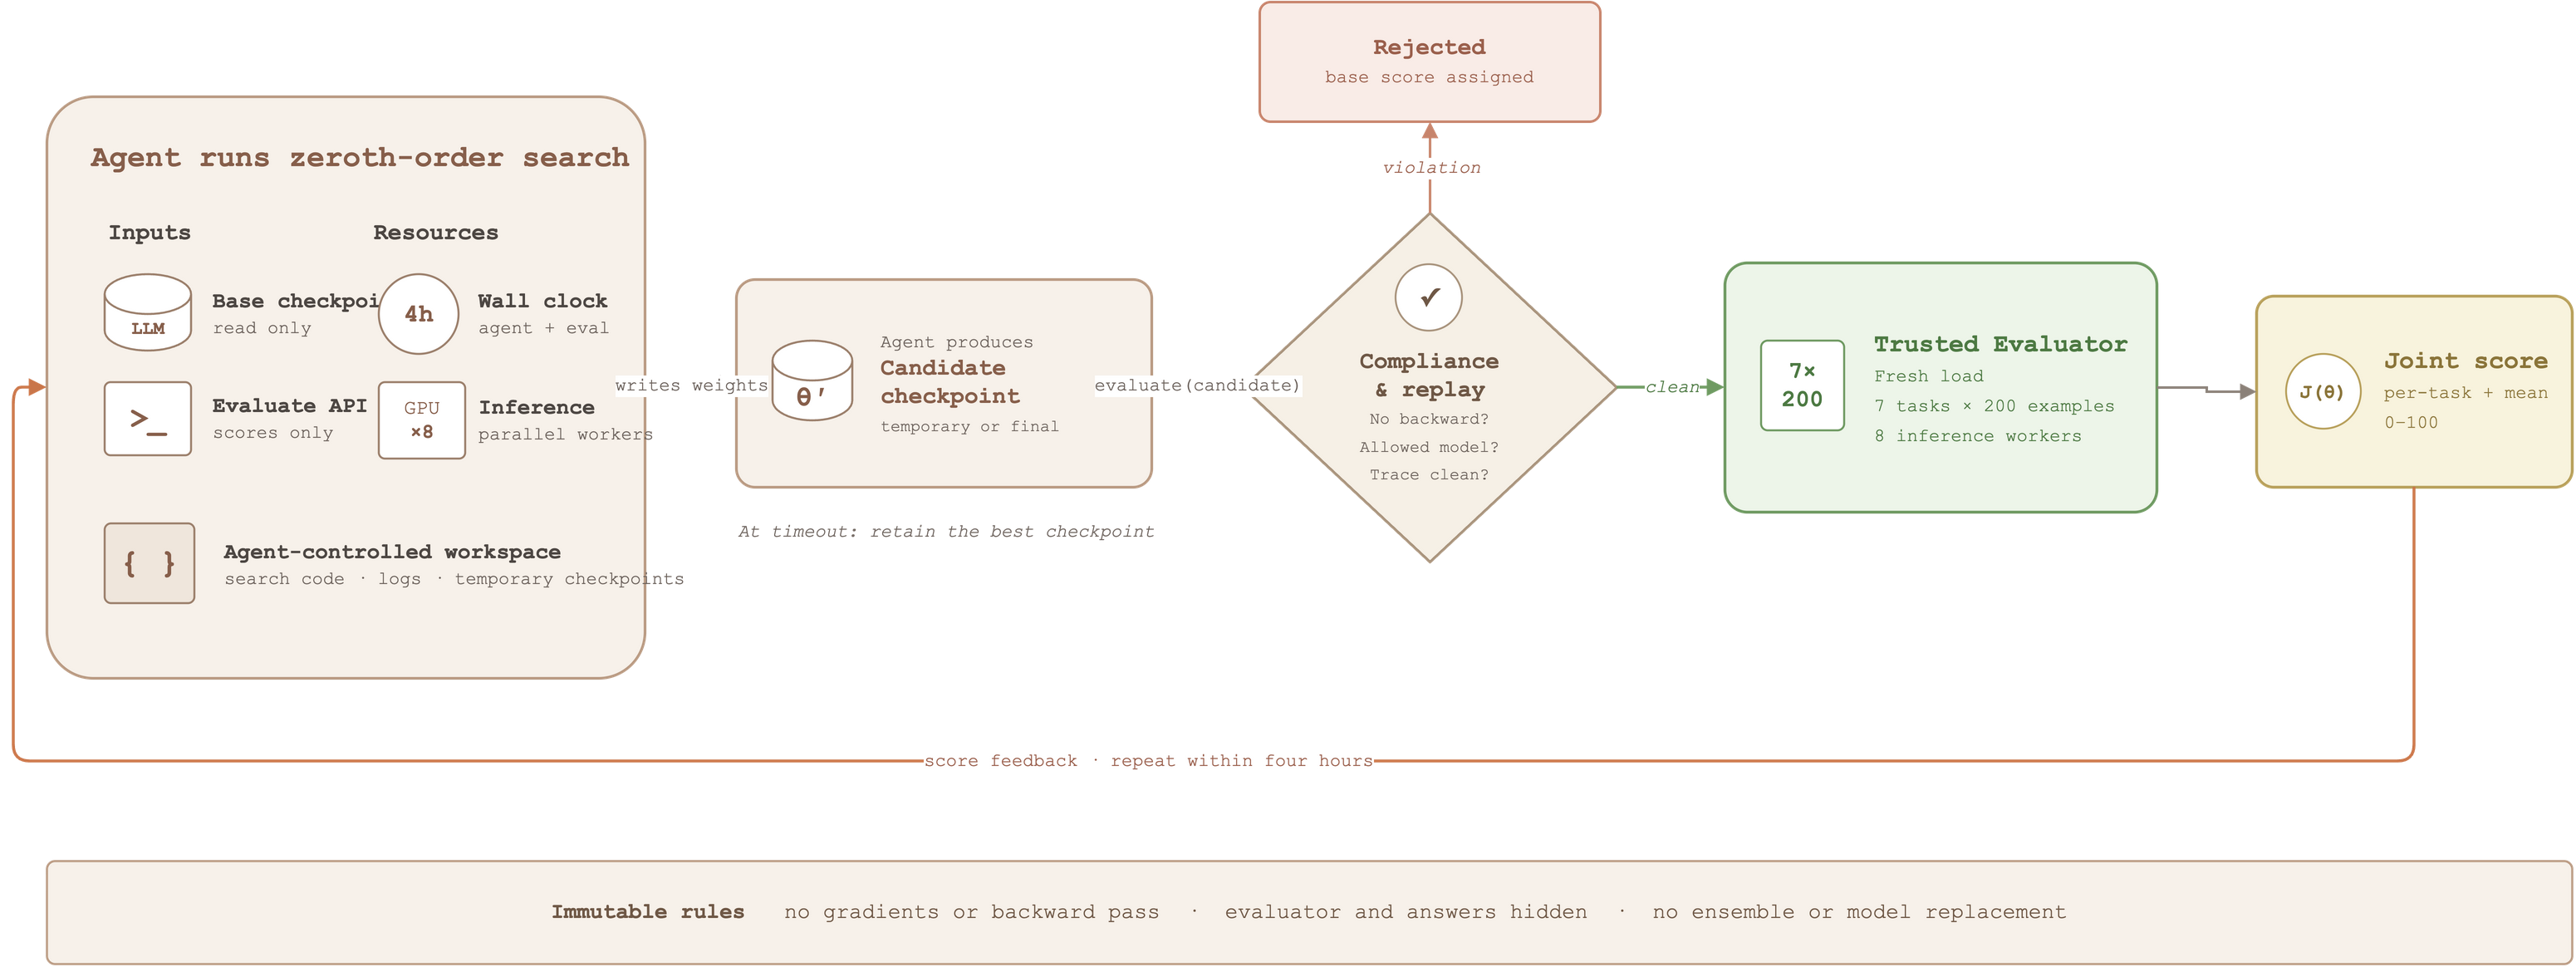
\includegraphics[width=\linewidth]{../docs/assets/system-overview.png}
    \caption{\textbf{\bench{} pipeline.} An agent receives a frozen base checkpoint,
    score-only evaluation access, and a four-hour compute budget. It iterates inside a
    writable workspace and produces one candidate checkpoint. A trusted audit rejects
    gradients, model substitution, evaluator access, and multi-model submission; valid
    checkpoints are reloaded in a fresh process and evaluated on all seven tasks.}
    \label{fig:system}
\end{figure}

Figure~\ref{fig:system} summarizes one episode. All harnesses receive the same instruction,
resources, candidate language, and evaluation commands. The underlying frontier model and
CLI scaffold together form the research agent: the model plans and interprets feedback,
while the scaffold manages tool calls, shell execution, files, permissions, and context.
We evaluate Codex CLI, Cursor Agent, and OpenCode without human intervention.

\subsection{Agent architecture and isolation}
All harnesses receive the same instruction and four commands: evaluate one candidate,
evaluate a batch, read completed results, and inspect remaining time. The agent can write
only inside a fresh workspace and reads the base checkpoint through a read-only mount.
Raw examples, labels, scorer code, trusted attempt history, credentials, and the final
checkpoint store remain outside the agent-visible filesystem. General network access is
disabled for agent-issued shell commands.

\subsection{Evaluation suite}
Each task contains 200 fixed examples. We use greedy decoding, generation seed 42, and
task-specific output limits. The suite covers constrained arithmetic (Countdown), grade
school mathematics (GSM8K), competition mathematics (MATH-500 and OlympiadBench), code
generation (MBPP), story ordering (ROCStories), and reaction classification (USPTO-50K).
The current experiments expose the same examples for search feedback and final replay.
Fresh replay verifies checkpoint integrity and score reproducibility; it does not establish
generalization to unseen examples. We therefore call all reported values \emph{visible
development scores}.

\subsection{Score-only model improvement}

Let $\theta_0$ be a frozen base checkpoint, let $\mathcal{T}$ be the seven-task suite,
and let $s_t(\theta)\in[0,100]$ be the deterministic score of checkpoint $\theta$ on
task $t$. The joint objective is
\begin{equation}
    \score(\theta)=\frac{1}{|\mathcal{T}|}\sum_{t\in\mathcal{T}}s_t(\theta).
    \label{eq:objective}
\end{equation}
At step $k$, the agent chooses a checkpoint $\theta_k$ using only its instruction,
workspace state, and the score history
$\mathcal{H}_{k-1}=\{(\theta_j,\{s_t(\theta_j)\}_{t\in Q_j}):j<k\}$, where
$Q_j\subseteq\mathcal{T}$ is the requested task subset. The evaluator returns task scores;
it does not return gradients, optimizer state, hidden labels, or training examples. The
episode output is the highest-scoring checkpoint among those evaluated on the complete
suite:
\begin{equation}
    \hat\theta_B=\arg\max_{\theta_k:\,Q_k=\mathcal{T}} \score(\theta_k),
    \qquad k\leq B,
    \label{eq:best-budget}
\end{equation}
where $B$ is not a fixed query count but the number of complete evaluations the agent can
finish within the wall-clock budget. This distinction matters: the protocol measures both
search decisions and the systems work needed to realize them. Eight GPUs provide
evaluation concurrency, but Equation~\ref{eq:best-budget} always selects one checkpoint;
scores never ensemble predictions from multiple models.

\subsection{Deterministic perturbation programs}

The measured implementation describes a candidate with a short perturbation program
$c=\{(z_i,\alpha_i,g_i)\}_{i=1}^{m}$:
\begin{equation}
    \theta(c)=\theta_0+\sum_{i=1}^{m}\alpha_i P_{g_i}u(z_i).
    \label{eq:candidate}
\end{equation}
Here $u(z_i)$ is the full-model Gaussian direction reproduced by the evaluator from seed
$z_i$, $\alpha_i\in\mathbb{R}$ is its signed scale, and $P_{g_i}$ optionally restricts the
direction to a named parameter group ($P_{g_i}=I$ for a full-model perturbation). Seeds are
therefore replay identifiers, not hidden scores or coordinates that an agent can interpret.
Composition ($m>1$) represents a new single checkpoint, rather than an ensemble.

Every call reconstructs Equation~\ref{eq:candidate} directly from $\theta_0$. It never
adds noise to the previously evaluated BF16 checkpoint. This exact-reset rule makes a
candidate's score a function of its program rather than its evaluation order and avoids
cumulative restoration error. Within this representation, an agent can sample independent
directions, compare antithetic pairs, move a search center by composing terms, change
scales, or replace both provided examples. The antithetic example follows the
score-difference intuition of evolution strategies \citep{salimans2017es}.

\subsection{What random search establishes}

For a fixed scale $\sigma$, the simplest reference policy samples independent seeds
$z_i$ and evaluates $\theta_i=\theta_0+\sigma u(z_i)$. Let
\begin{equation}
    p_\sigma=\Pr_z[\score(\theta_0+\sigma u(z))>\score(\theta_0)]
    \label{eq:improvement-probability}
\end{equation}
measure local improvability, and let
\begin{equation}
    M_N(\sigma)=\max_{1\leq i\leq N}\score(\theta_0+\sigma u(z_i))
    \label{eq:best-of-n}
\end{equation}
be the best score under an $N$-candidate random budget. If samples are independent, the
probability of finding at least one improvement is
$1-(1-p_\sigma)^N$. Thus $p_\sigma>0$ establishes that useful checkpoints exist nearby,
but a best-of-run score is not by itself evidence of an intelligent policy: even unchanged
random search improves as $N$ grows. We consequently report the distribution of
$M_N(\sigma)$, candidate count, and search traces alongside each endpoint.

\section{Preliminary: Is Random Search a Meaningful Task?}

Before comparing agents, we first establish what can and cannot be obtained by independent
random sampling. This preliminary serves two purposes. It verifies that useful checkpoints
exist in the permitted neighborhood, and it measures how much score can be attributed to
the number of random trials alone. We estimate Equations~\ref{eq:improvement-probability}
and~\ref{eq:best-of-n} on Qwen2.5-3B-Instruct. We evaluate 1,000 independently reconstructed
full-model candidates at $\sigma=5\times10^{-4}$. The empirical local-improvement rate is
$\hat p_\sigma=354/1000=0.354$: improvement over the 44.08 base is feasible and is not a
rare event at this scale. The fixed Random-500 baseline selects the best joint checkpoint
among the first 500 candidates and reaches 45.89; the strongest candidate in the full pool
reaches 46.80. Figure~\ref{fig:premise}B
then resamples the same fixed pool to show how the median and 10th--90th percentile of
$M_N(\sigma)$ change with $N$. The increasing curve quantifies the advantage obtained from
candidate count alone.

\begin{figure}[H]
    \centering
    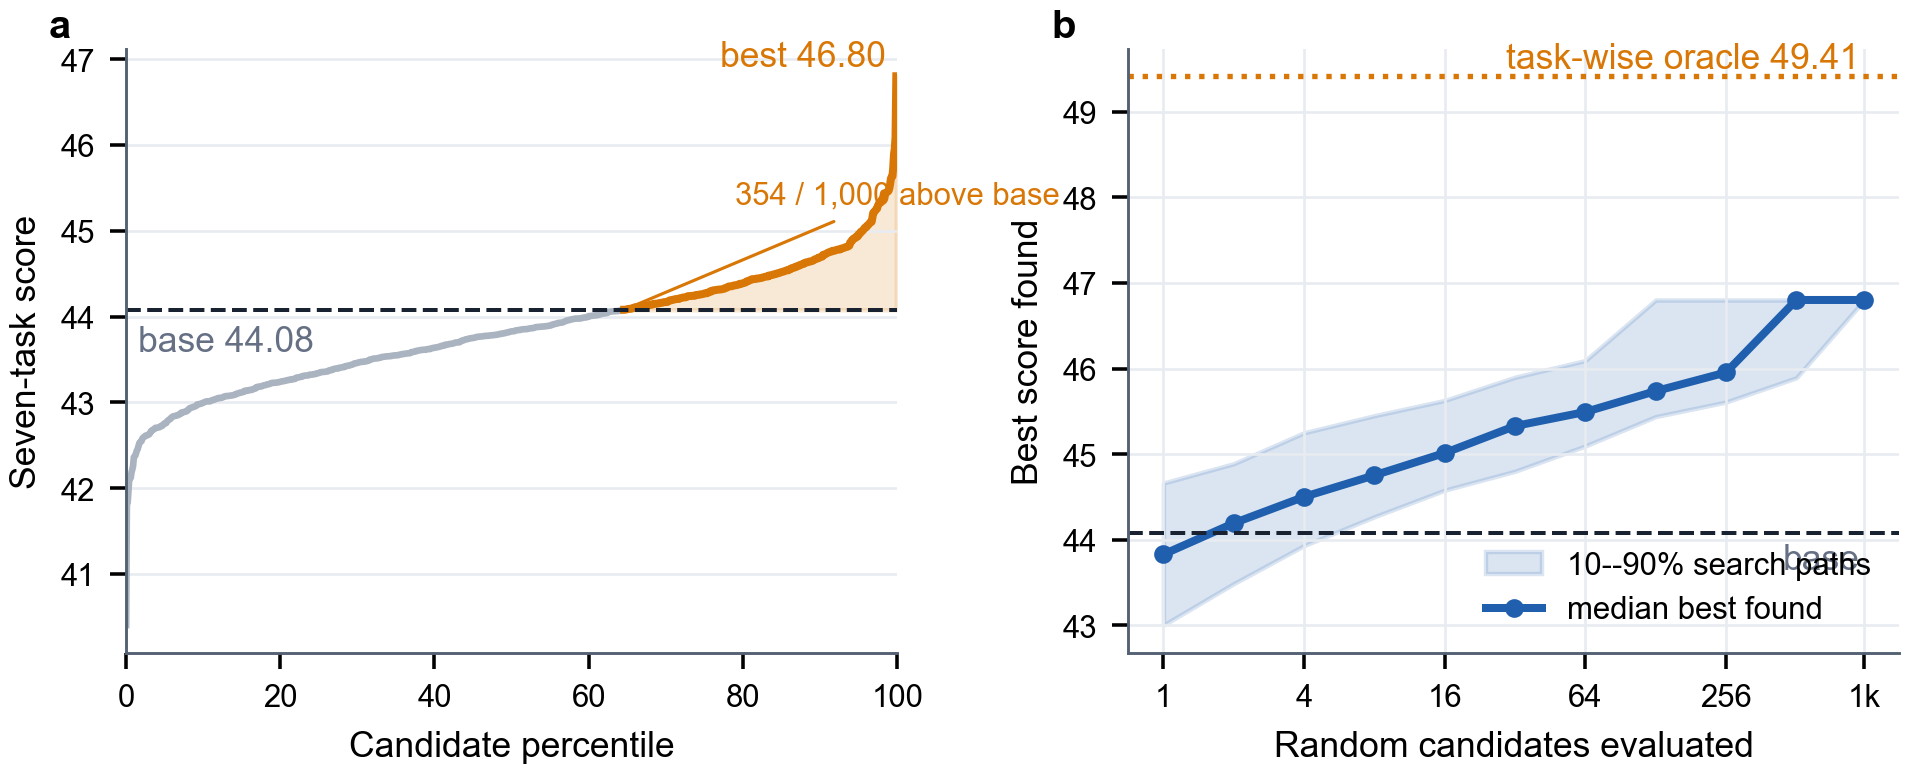
\includegraphics[width=\linewidth]{figures/fig2-search-space.pdf}
    \caption{\textbf{The local search space contains signal and substantial best-of-$N$
    variation.} (A) All 1,000 exact-reset Qwen2.5-3B candidates sorted by joint score.
    (B) Expected best score after $N$ random candidates, estimated from 2,000 random
    permutations of the fixed pool; the band contains the 10th--90th percentiles. More
    evaluations improve the expected maximum even without a better search strategy.}
    \label{fig:premise}
\end{figure}

\subsection{Projected structure of the weight neighborhood}

The 1,000 candidates are points in a parameter space with billions of dimensions. Following
the diagnostic used by Neural Thickets, we map every score-independent perturbation into
the same two-dimensional random projection and interpolate only for visualization
\citep{gan2026neuralthickets}. Figure~\ref{fig:landscape} shows the joint objective and all
seven tasks at exactly the same sampled coordinates. Each panel also reports the largest
observed gain and how many of the 1,000 perturbations beat the frozen checkpoint on that
task. Red and blue regions interchange across panels: a direction that is locally favorable
for GSM8K can be neutral or harmful for Countdown or MBPP. This projected landscape
supplies the geometric intuition for random sampling:
the search window contains many distinct favorable pockets, yet no single direction is
uniformly favorable. The interpolated surface is a visual summary of measured samples, not
an estimate of the true billion-dimensional loss surface.

The panel statistics make the asymmetry concrete. Of the same 1,000 candidates, 650 beat
the MBPP base and 610 beat the GSM8K base, but only 147 beat the ROCStories base and 206
beat the Countdown base. The largest task-specific gain ranges from $+1.5$ points on
ROCStories to $+8.5$ on MBPP. More importantly, the gold stars occupy different locations:
the best candidate for one task is generally not the best candidate for another. The joint
panel compresses these competing effects: 356 candidates improve the seven-task average,
and the best joint gain is $+2.7$ points.

\begin{figure}[H]
    \centering
    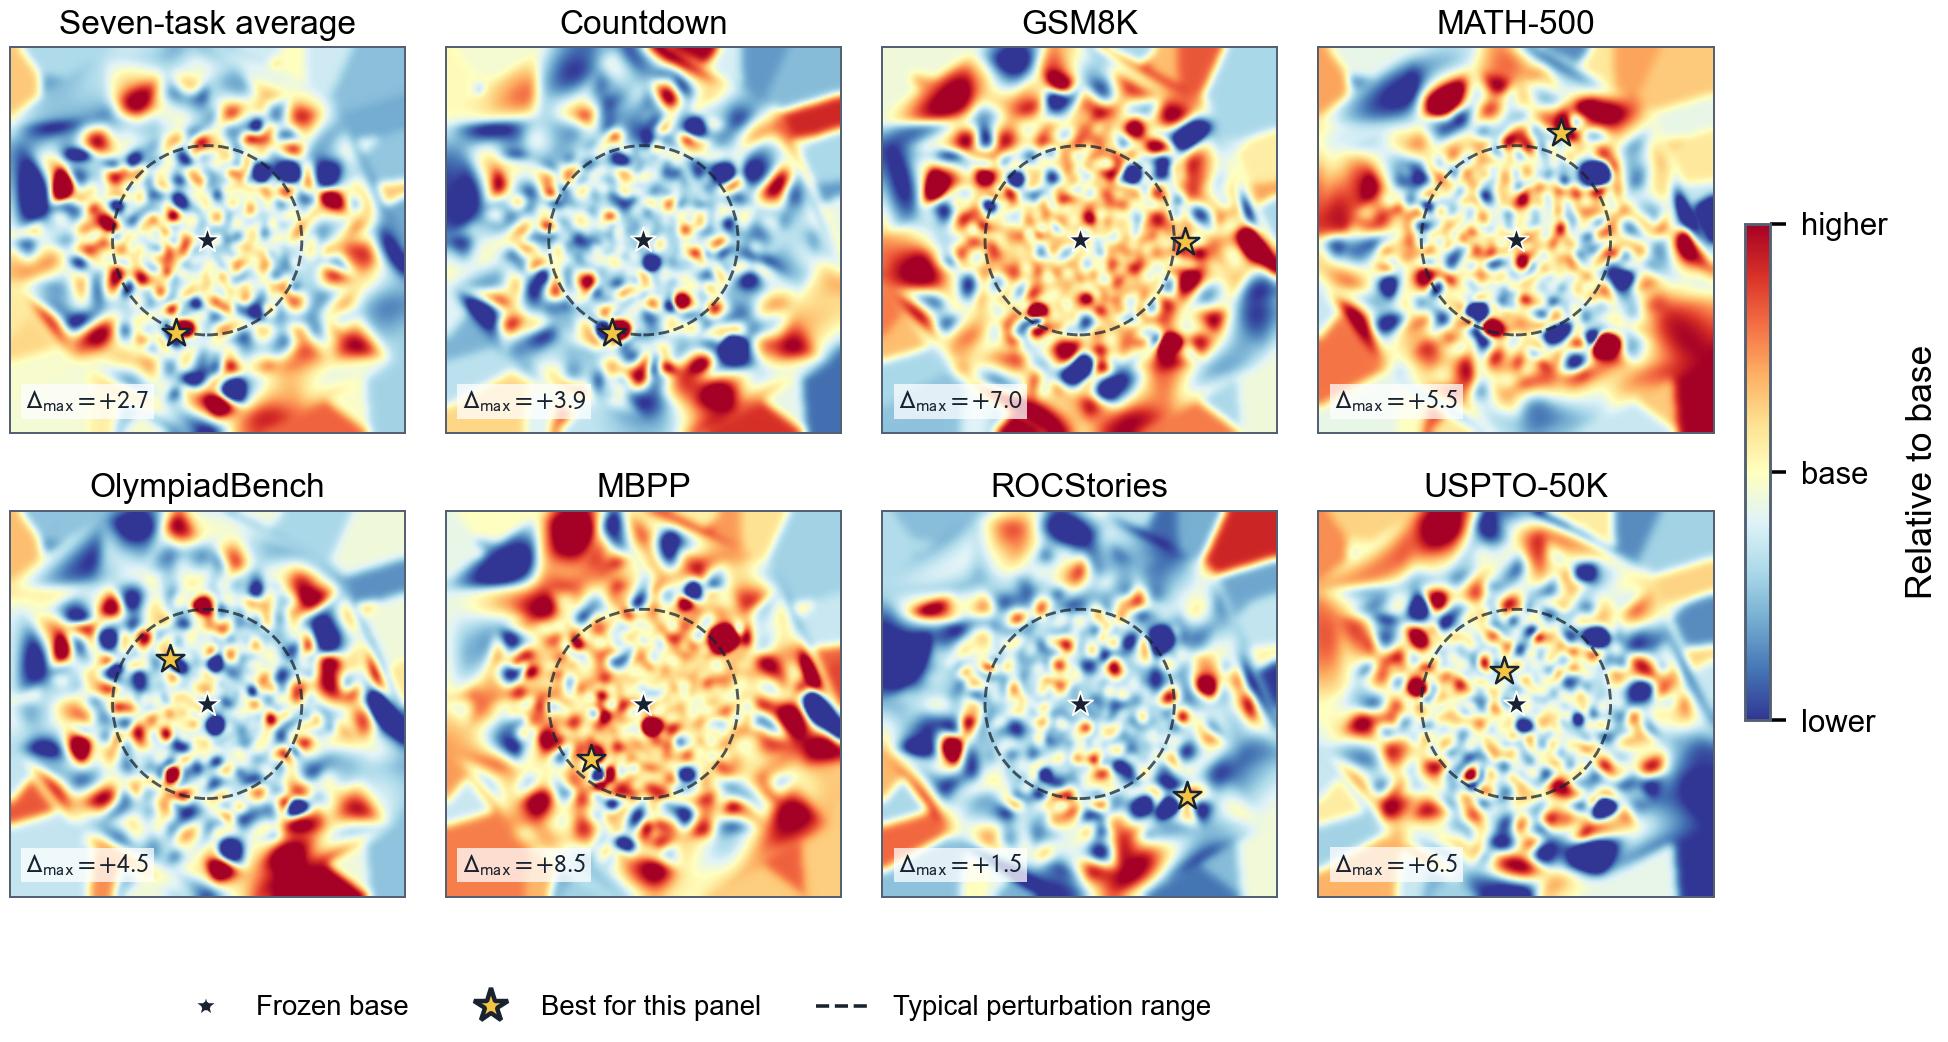
\includegraphics[width=\linewidth]{figures/fig3-weight-space-landscape.pdf}
    \caption{\textbf{Accuracy landscapes from 1,000 random perturbations of the primary
    Qwen2.5 target.} All panels use the same score-blind random projection. Color represents
    task-normalized change from the frozen checkpoint (blue: lower; white: base; red:
    higher). Every panel prints its best gain and the number of candidates above base. The
    black star is the base, the gold star is the best sampled perturbation for that panel,
    and the dashed circle marks the typical projected perturbation range.}
    \label{fig:landscape}
\end{figure}

\subsection{Why a joint checkpoint is harder than a task specialist}

A task-wise oracle that may select a different checkpoint for each task scores 49.41,
which is 2.61 points above the best legal single checkpoint. To locate the source of this
gap, for each task we take its highest-scoring checkpoint and inspect that checkpoint on
the other six tasks. Figure~\ref{fig:conflict} shows strong diagonal gains but frequent
off-diagonal losses. Most candidates improve two to four tasks, twelve improve six, and
none improves all seven. The preliminary therefore establishes three properties needed by
the benchmark: improvements exist, finite-budget outcomes vary, and task-specialist gains
do not automatically compose into one jointly strong checkpoint.

\begin{figure}[H]
    \centering
    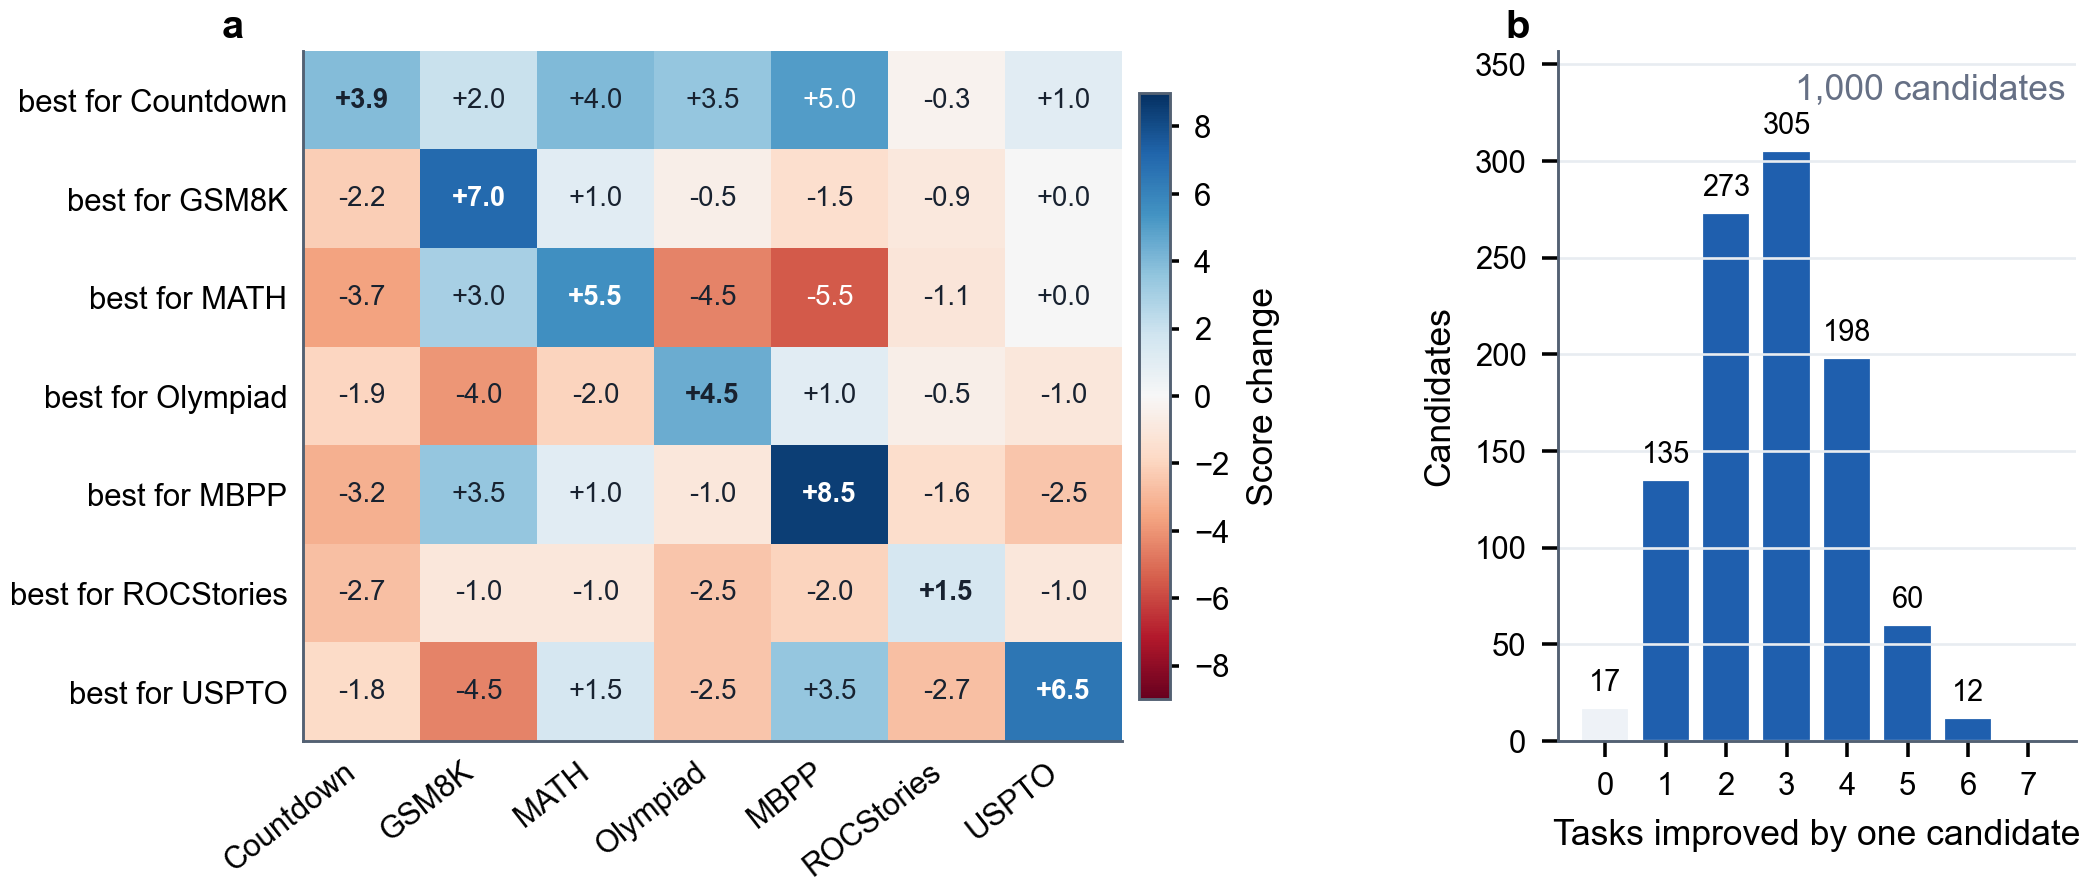
\includegraphics[width=\linewidth]{figures/fig4-task-conflict.pdf}
    \caption{\textbf{The joint objective contains genuine task conflict.} (A) Per-task
    changes for seven specialist checkpoints, each selected only by the row task.
    (B) Number of tasks improved by every candidate in the 1,000-point pool. No sampled
    checkpoint improves all seven tasks.}
    \label{fig:conflict}
\end{figure}

\FloatBarrier
\section{Agent Experiments}

Qwen2.5-3B-Instruct is the primary target; its unmodified joint score is 44.08. Each
episode lasts four hours and exposes eight H20 GPUs for parallel inference. Reasoning,
code execution, evaluator calls, and checkpoint handling all count toward the wall-clock
budget. We call a run \emph{score-bearing} when it completes at least one evaluation over
all seven tasks. A missing final submission does not erase such an observation: we retain
the highest complete seven-task score reached during the run and report checkpoint replay
and audit status separately. For a balanced primary comparison, we keep the three highest
score-bearing runs for each of 13 exact agent--harness--reasoning settings, yielding 39
displayed runs. The stricter trace analysis uses the 31 runs that also pass audit and fresh
checkpoint replay.

The target-model ablation repeats the same protocol for 16 score-bearing episodes on Qwen3-4B-Base,
whose unmodified score is 41.08. This is a standard part of the experimental design: it
tests whether findings on the primary checkpoint persist after changing the frozen target
and its local weight geometry. Eight exact settings have two same-protocol runs each.
Scores and ranks are reported separately for the two targets.

\FloatBarrier
\section{Results}

We first ask whether agents improve the primary Qwen2.5 checkpoint and how they search its
neighborhood. We then change only the target checkpoint in an auxiliary ablation.

\subsection{Main results}

Table~\ref{tab:main} reports the balanced primary comparison together with the fixed
Random-500 baseline. GPT-5.5 high reaches the highest retained-run mean (48.39), followed
by Kimi K2.6 (48.09) and GPT-5.5 xhigh (47.98), compared with 44.08 for the base
checkpoint. Every configuration reaches an improving candidate. The table measures the
high-score region each setting reached under repeated four-hour search; because settings
with more historical runs are truncated to their three highest scores, it is not an
unbiased estimate of full-run success probability. Complete run records and audit fields
are retained separately.

\begin{table}[t]
\centering
\small
\setlength{\tabcolsep}{7pt}
\caption{\textbf{Primary results on Qwen2.5-3B-Instruct (0--100).} Each agent row uses
the three highest score-bearing runs for one exact model, harness, and reasoning setting.
A score-bearing run contributes its best complete seven-task score even if final submission
failed; audit-valid replay is analyzed separately. Random-500 selects the best joint
checkpoint from one fixed sequence of 500 independent perturbations.}
\label{tab:main}
\begin{tabular}{llrrr}
\toprule
System & Harness & Mean & $\Delta$ Base & Range \\
\midrule
GPT-5.5 high & Codex & \textbf{48.39} & \textbf{+4.32} & 47.56--49.23 \\
Kimi K2.6 & OpenCode & 48.09 & +4.02 & 47.51--49.25 \\
GPT-5.5 xhigh & Codex & 47.98 & +3.91 & 47.66--48.17 \\
GPT-5.6 medium & Codex & 47.72 & +3.65 & 46.69--48.83 \\
GPT-5.6 xhigh & Codex & 47.59 & +3.52 & 46.81--48.64 \\
GPT-5.6 high & Codex & 46.84 & +2.77 & 46.27--47.28 \\
DeepSeek V4 Pro & OpenCode & 46.56 & +2.48 & 45.62--47.11 \\
Opus 4.8 high & Cursor & 46.42 & +2.35 & 46.04--47.13 \\
Sonnet 4.6 medium & Cursor & 46.41 & +2.33 & 45.59--47.92 \\
GPT-5.4 Pro & OpenCode & 46.09 & +2.02 & 45.61--46.83 \\
MiniMax M2.7 & OpenCode & 46.09 & +2.01 & 45.40--47.12 \\
GLM-5.1 & OpenCode & 45.99 & +1.91 & 45.88--46.19 \\
Qwen3.7-Max & OpenCode & 45.98 & +1.90 & 45.70--46.15 \\
\midrule
Random-500 & Fixed search & 45.89 & +1.81 & -- \\
\emph{Base checkpoint} & -- & 44.08 & 0.00 & -- \\
\bottomrule
\end{tabular}
\end{table}

Across the 39 displayed primary runs, every setting contributes three scores above the
base checkpoint. Retained-run means gain 1.90--4.32 points, but the ranges overlap
substantially. The experiment therefore establishes broad feasibility more strongly than
a stable ordering: multiple research agents use the same score-only interface to locate
improvements, while differing in efficiency, composition behavior, and path stability.

\subsection{Target-model ablation}

We repeat the protocol for 16 episodes on Qwen3-4B-Base. Every tested configuration
improves the 41.08 base score, with mean gains between 3.42 and 7.92 points. The larger
improvements show that the benchmark is not tied to Qwen2.5, while also confirming that
the attainable gain depends on the local neighborhood of the target checkpoint. We keep
this experiment separate from the primary table and report its full matrix in
Appendix~\ref{app:qwen3}.

The eight settings shared by both targets have only weakly aligned retained-run gains
(Spearman $\rho=0.29$; Figure~\ref{fig:target-dependence}A). Target choice also changes
variance: GPT-5.6 xhigh spans 1.83 points on Qwen2.5 but 9.90 points on Qwen3, while
MiniMax spans 1.72 and 0.13 points, respectively. The ordering therefore reflects an
interaction between the research agent and the local geometry of the checkpoint being
optimized, rather than a target-independent agent capability score.

\begin{figure}[t]
    \centering
    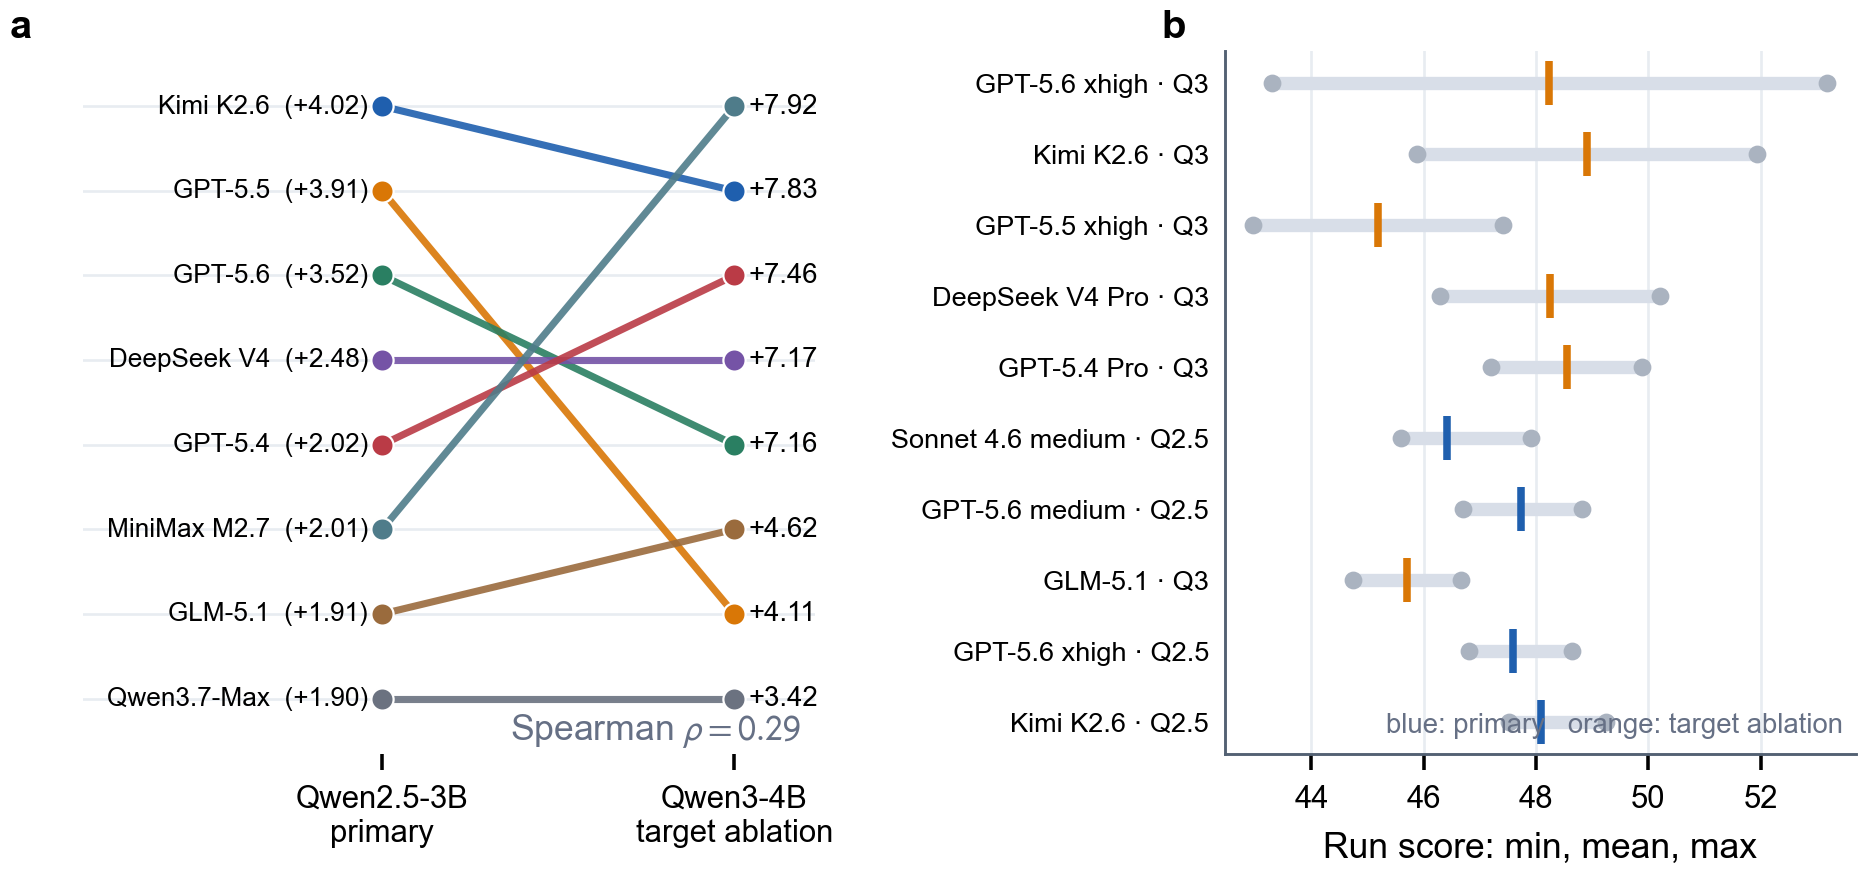
\includegraphics[width=\linewidth]{figures/fig3-target-dependence.pdf}
    \caption{\textbf{Agent outcomes depend strongly on the target checkpoint.} (A) Rank
    changes for the eight settings shared by the primary and auxiliary targets; labels
    report mean gain over the corresponding base. (B) The ten largest retained-run ranges
    across both targets. Blue ticks denote Qwen2.5 means and orange ticks denote Qwen3
    means; gray endpoints mark the observed minimum and maximum.}
    \label{fig:target-dependence}
\end{figure}

\subsection{Where the joint-score gains come from}

Figure~\ref{fig:tasks} compares Random-500 with all nine agent configurations for which a
fresh replay provides complete seven-task scores. Random search mainly improves GSM8K and MATH-500,
whereas agents discover qualitatively different trade-offs. Kimi K2.6 improves GSM8K,
MBPP, and USPTO-50K together; Opus 4.8 obtains the largest Countdown gain; and the GPT-5.6
configurations spread smaller positive changes across most tasks. Joint-score improvement
therefore does not correspond to one universal perturbation direction.

\begin{figure}[t]
    \centering
    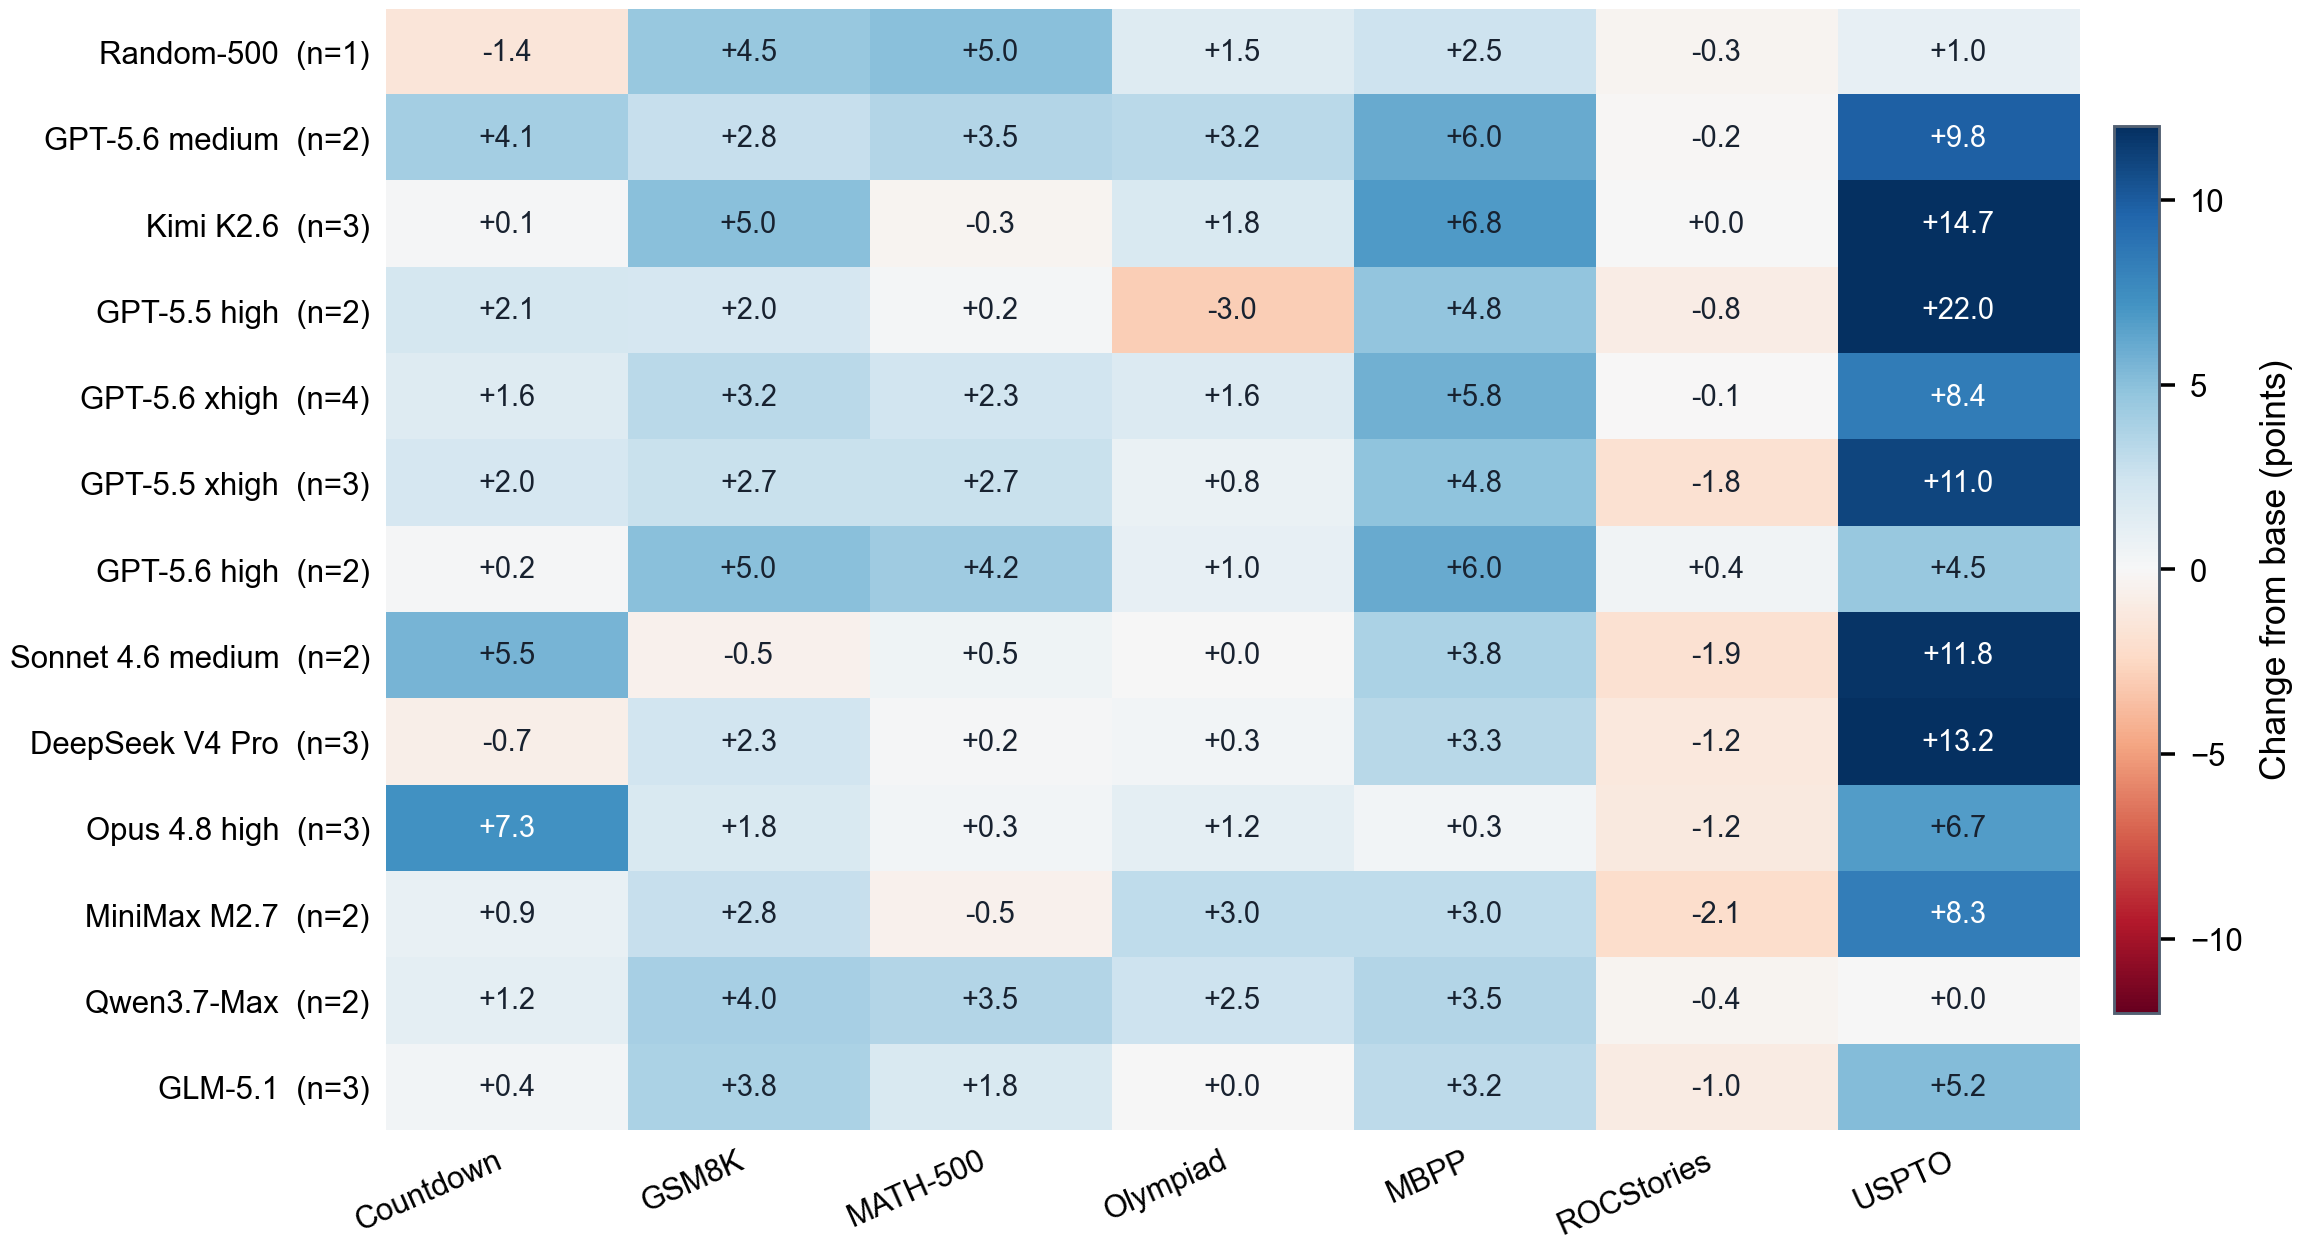
\includegraphics[width=\linewidth]{figures/fig4-task-breakdown.pdf}
    \caption{\textbf{Task-level changes on the primary Qwen2.5 target.} Cells show
    percentage-point change from the frozen checkpoint. Random-500 is the best joint
    checkpoint in the fixed 500-candidate sequence; the nine agent rows include every
    configuration with audit-valid per-task replay, with the number of runs printed beside
    its name.}
    \label{fig:tasks}
\end{figure}

\section{Agent Behavior Analysis}

Aggregate scores show what checkpoint was found; the retained traces show how it was found.
We analyze two complementary trace collections. The structured Qwen2.5 inventory contains
candidate statistics for 31 audit-valid agent runs. A matching trajectory export contains
31 audit-valid agent episodes with timestamped score histories. Fixed RandOPT and evolution-strategy
runs are excluded from the statistics in this section and discussed separately below.

\subsection{Time utilization}

The 31 audit-valid agents complete between 123 and 1,241 evaluations (median 427).
Candidate count matters---Figure~\ref{fig:premise} shows that the random-search maximum
grows with budget---but the traces contain more than repeated independent sampling. Agents
change scales, screen task subsets, compare directions, and move the search center during
the episode.

Long-horizon execution is consequential rather than ceremonial. For each of the 31
audit-valid timestamped agent runs, we measure when its running best first reaches 90\% of
its eventual gain over the base. The median is 147 minutes; 22 of 31 runs cross this
threshold after two hours, and 12 cross it after three hours (Figure~\ref{fig:behavior}A). Shortening the episode
to one hour would therefore remove much of the adaptive part of the task and favor agents
that happen to find a strong first batch.

\begin{figure}[t]
    \centering
    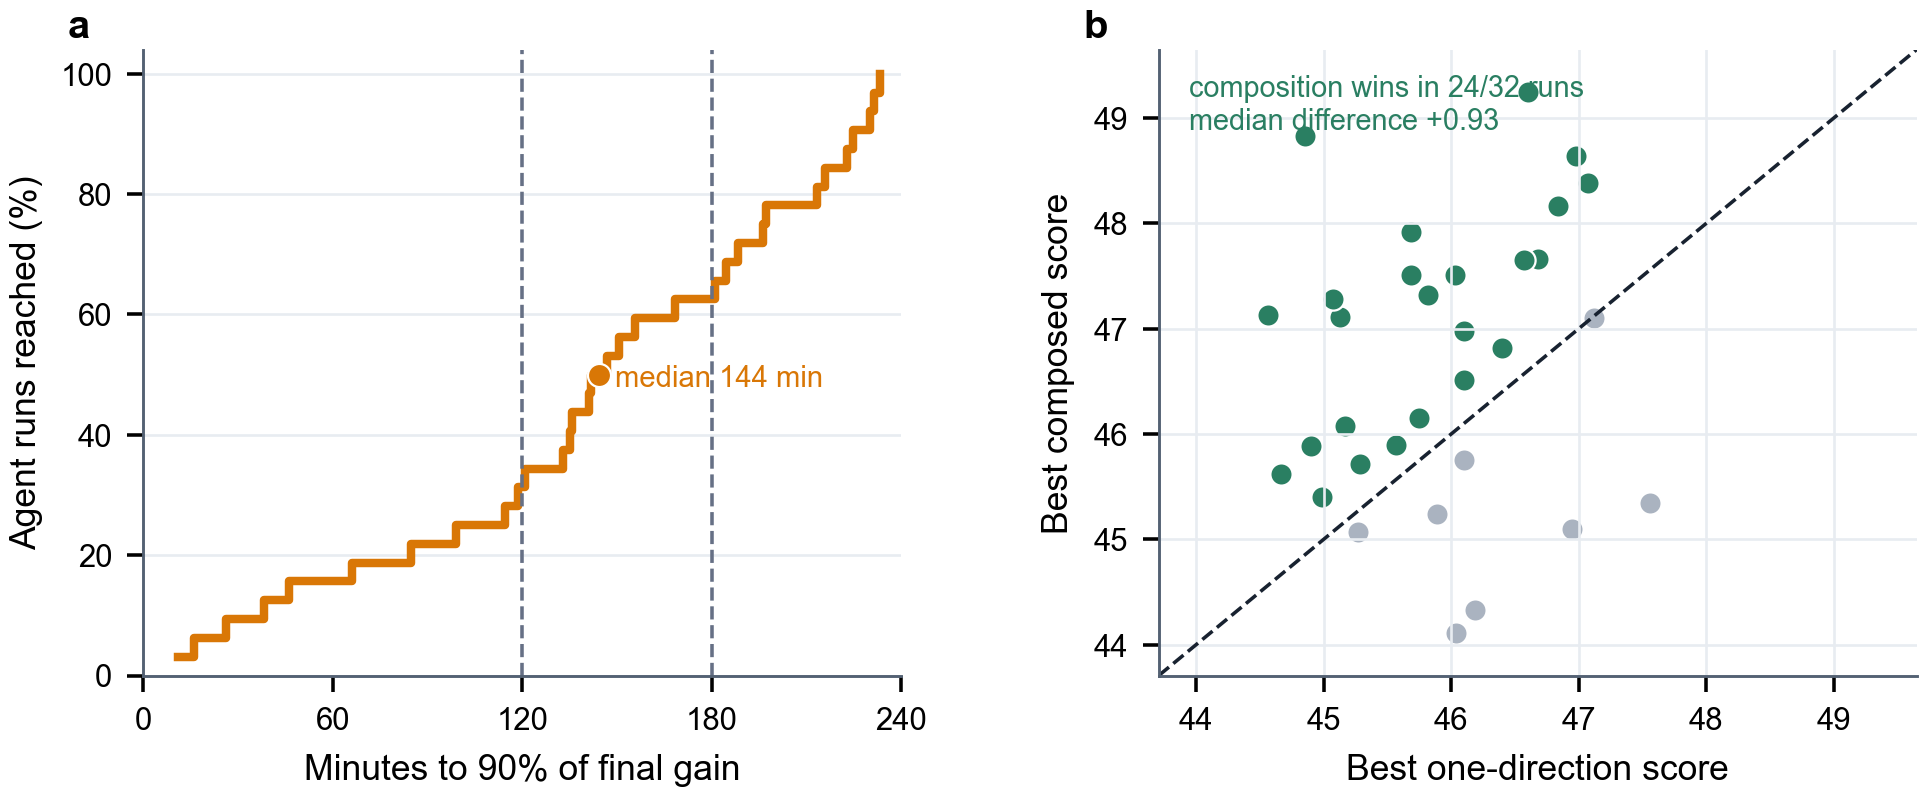
\includegraphics[width=\linewidth]{figures/fig6-agent-behavior.pdf}
    \caption{\textbf{What the complete traces reveal.} (A) Empirical time at
    which 31 audit-valid agent trajectories reach 90\% of their final gain; useful improvements continue
    throughout the four-hour horizon. (B) Best composed checkpoint versus best one-direction checkpoint
    within each audit-valid run. Composition wins in 24 of 31 runs.}
    \label{fig:behavior}
\end{figure}

\subsection{Search strategy and checkpoint composition}

The clearest strategic distinction is whether an agent merely samples independent
directions or turns earlier feedback into a new search center. A composed checkpoint wins
in 24 of 31 audit-valid runs, and the median difference between each run's best composed
and best one-direction checkpoint is $+0.95$ points (Figure~\ref{fig:behavior}B). The
pattern is agent-dependent: all three Kimi K2.6 runs and all eight valid GPT-5.6 runs finish
with composed checkpoints, compared with one of three Opus runs and one of three GLM runs.
This does not prove that composition is universally better---seven runs favor a single
direction---but it identifies a concrete behavior that endpoint-only leaderboards hide.

To compare concrete policies rather than averaged behaviors, Figure~\ref{fig:search-styles}
selects the highest-scoring audit-valid Qwen2.5 run for each of nine agent configurations.
Panel A shows
the running best score. Panel B separates one-direction candidates
$\theta_0+\alpha z$ from composed candidates
$\theta_0+\sum_i\alpha_i z_i$ and reports the number $k$ of directions in the selected
checkpoint. This best-run view diagnoses what each agent can discover; the means and ranges
in Table~\ref{tab:main} remain the appropriate evidence for stability.

The policies differ sharply. Kimi and GPT-5.6 xhigh devote roughly 70\% of their candidate
programs to composition and select three- and four-direction checkpoints, respectively.
GPT-5.5 high and xhigh remain probe-heavy, whereas GPT-5.6 high and Opus devote more than
95\% of classified programs to composition and select nine-direction checkpoints. Sonnet
divides its search almost evenly between the two operation classes, while DeepSeek remains
probe-heavy but obtains its best score from four combined directions. Thus, similar
endpoint scores can be reached through substantially different uses of the evaluator
budget.

\begin{figure}[H]
    \centering
    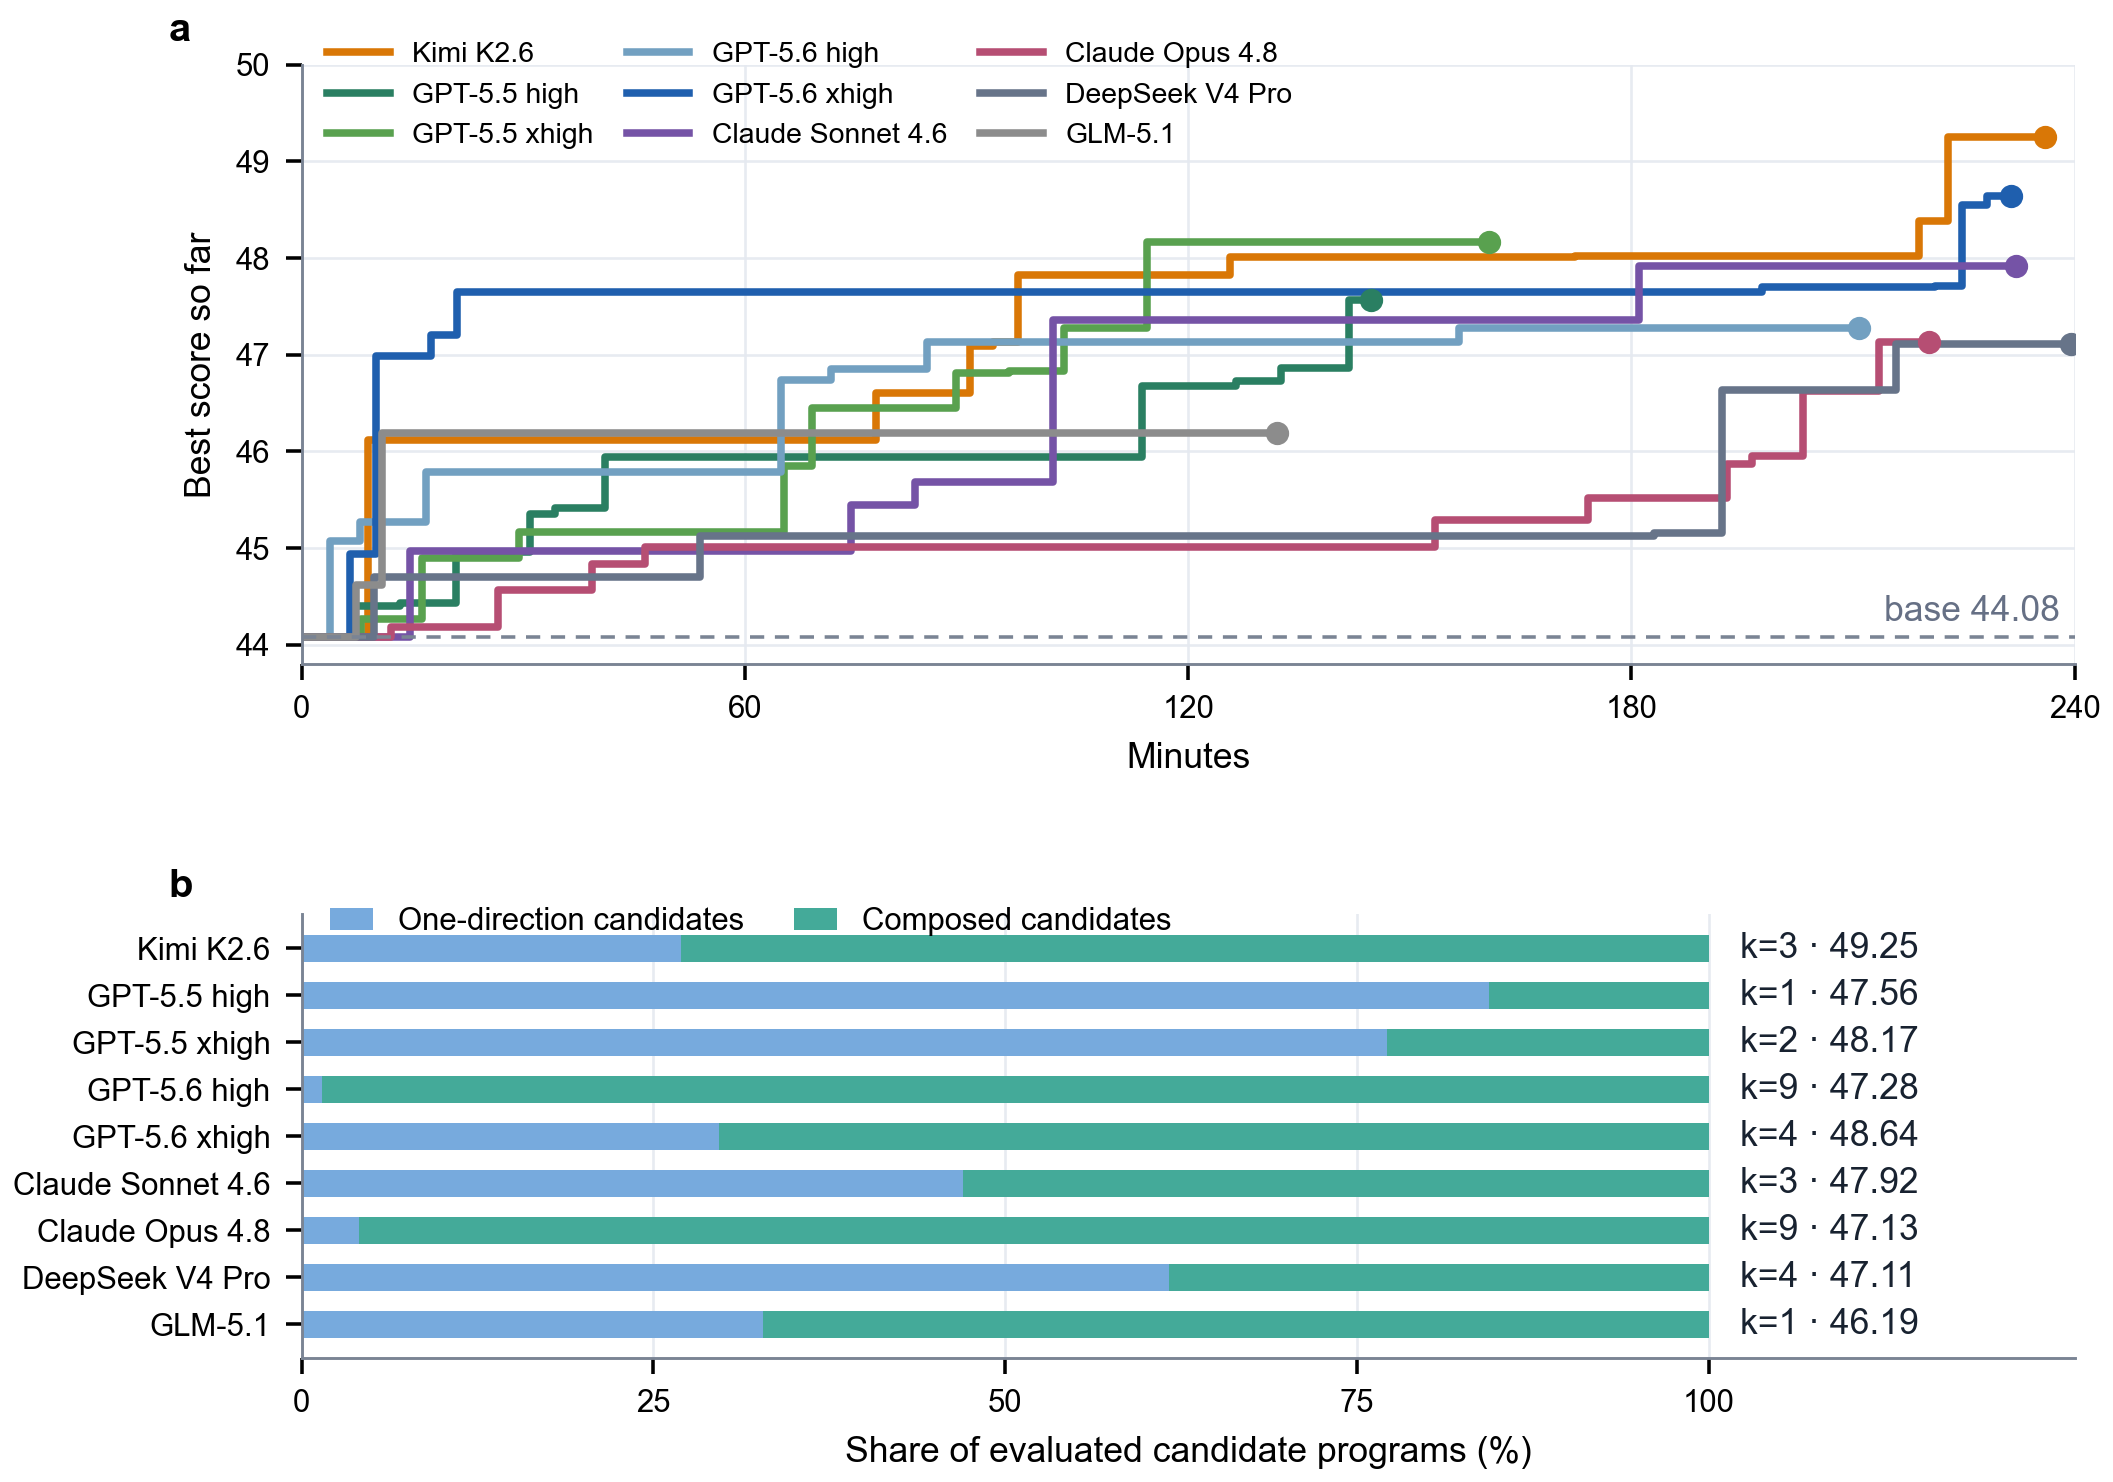
\includegraphics[width=\linewidth]{figures/fig6b-best-run-search-styles.pdf}
    \caption{\textbf{Best-run search behavior differs across agent configurations.} For
    each of the nine configurations with audit-valid detailed traces, we select its
    highest-scoring run on Qwen2.5-3B-Instruct. (A) Running best
    seven-task score over the four-hour episode. Dots mark the final best observed score.
    (B) Share of classified candidate programs using one perturbation direction versus a
    linear combination of multiple directions. The right annotation gives the number of
    directions $k$ in the best checkpoint and its score. The figure describes search
    behavior within selected best runs; Table~\ref{tab:main} reports repeated-run means.}
    \label{fig:search-styles}
\end{figure}

The aggregate counts above do not reveal what an agent actually wrote into its checkpoint.
Figure~\ref{fig:operations} therefore reconstructs the exact best checkpoint from every
selected run in a common executable notation. Each \texttt{noise(seed)} call regenerates
one deterministic full-model Gaussian direction, and each signed coefficient is the scale
recorded in the trace. The six programs expose qualitatively different decisions. Kimi
keeps three positive directions; GPT-5.6 combines one dominant negative direction with
three smaller signed corrections; GPT-5.5 high selects one negative direction; Sonnet and
DeepSeek use short signed compositions; and Opus accumulates nine directions. These are
the concrete model edits behind the curves in Figure~\ref{fig:search-styles}, not inferred
labels or post-hoc strategy names.

\begin{figure}[t]
    \centering
    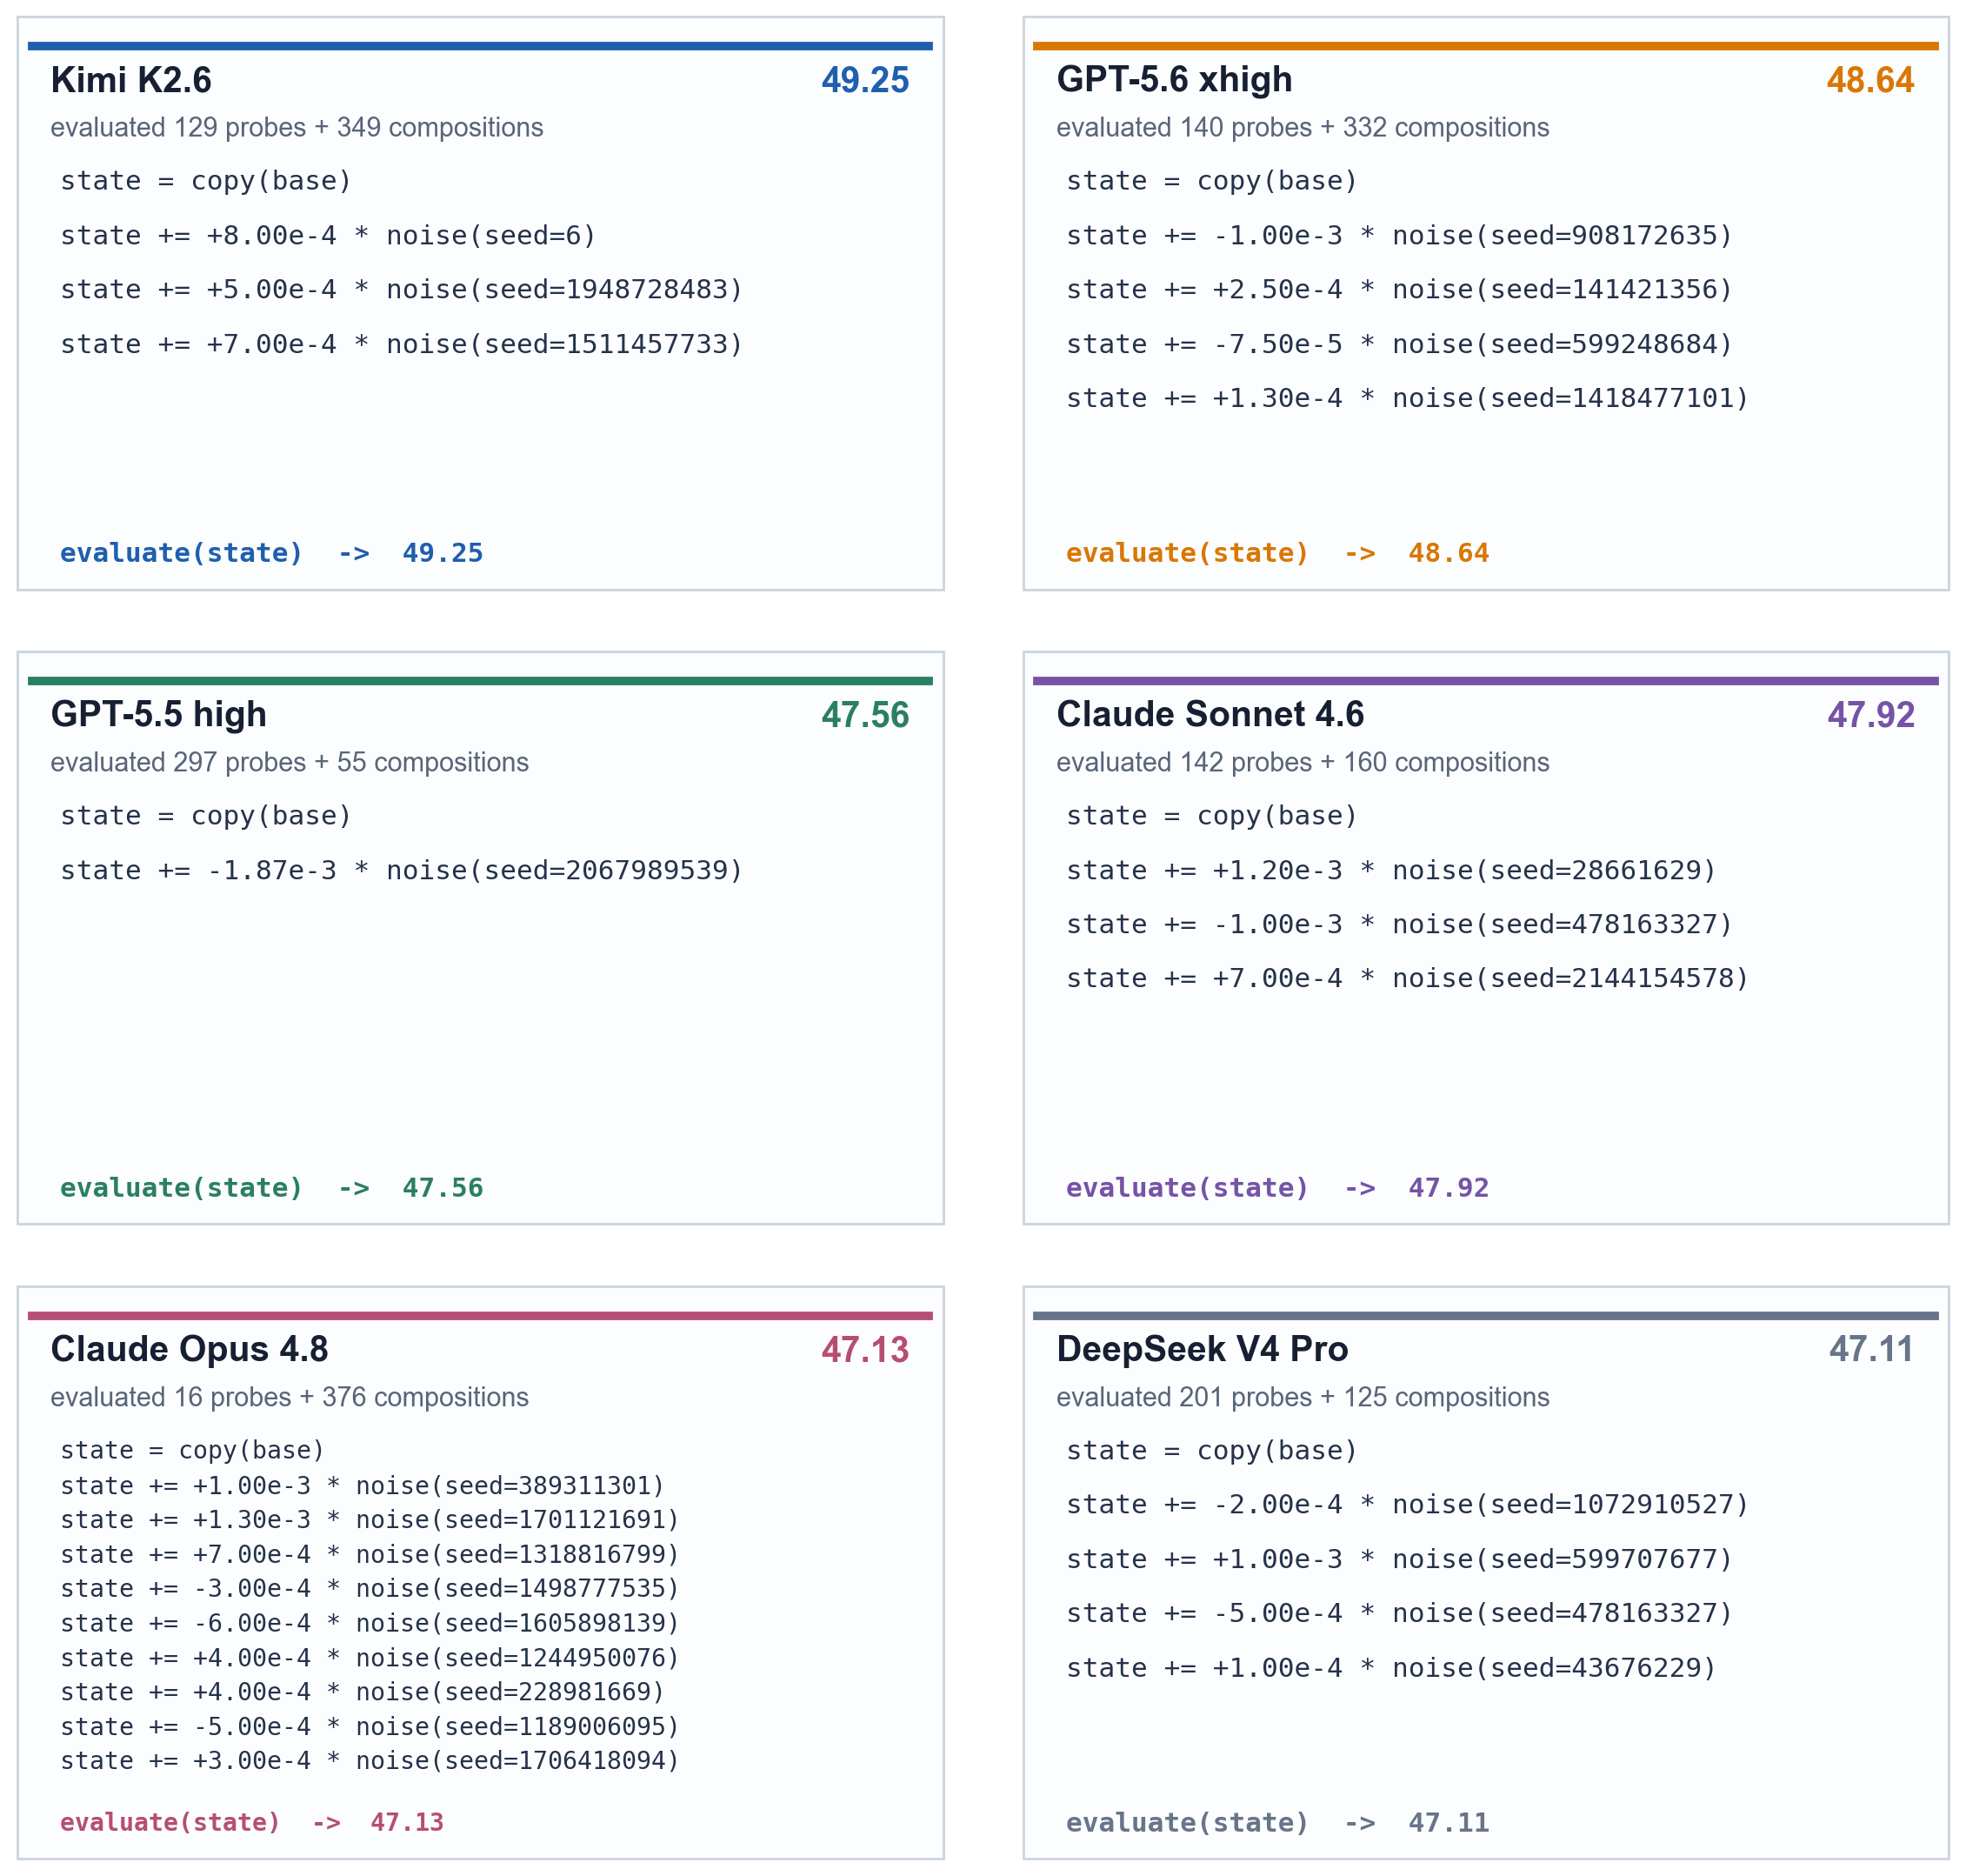
\includegraphics[width=\linewidth]{figures/fig6c-concrete-agent-operations.pdf}
    \caption{\textbf{Exact operations that construct each selected best checkpoint.}
    We replay the highest-scoring complete Qwen2.5-3B-Instruct run for each agent in one
    normalized notation: copy the frozen base, add every recorded seeded direction at its
    recorded scale, and evaluate the resulting state. The header reports the total number
    of one-direction probes and composed candidates evaluated during that run. The snippets
    are exact reconstructions of checkpoint specifications; they are not claimed to be
    verbatim source code written by the agent.}
    \label{fig:operations}
\end{figure}

Figure~\ref{fig:walks} places the three complete Qwen3 ablation traces with retained
checkpoint programs into the same visual language. Within each episode, perturbation
programs are projected through one common,
score-independent Gaussian basis; the background interpolates that run's measured joint
scores, while arrows connect evaluations in execution order. The coordinates summarize
the program terms and are not exact BF16 tensor differences. GPT-5.5 stays in a tight
neighborhood, GLM-5.1 makes large exploratory jumps before returning toward the base, and
MiniMax concentrates later evaluations near a displaced center. Endpoint score alone
discards this structure.

\begin{figure}[t]
    \centering
    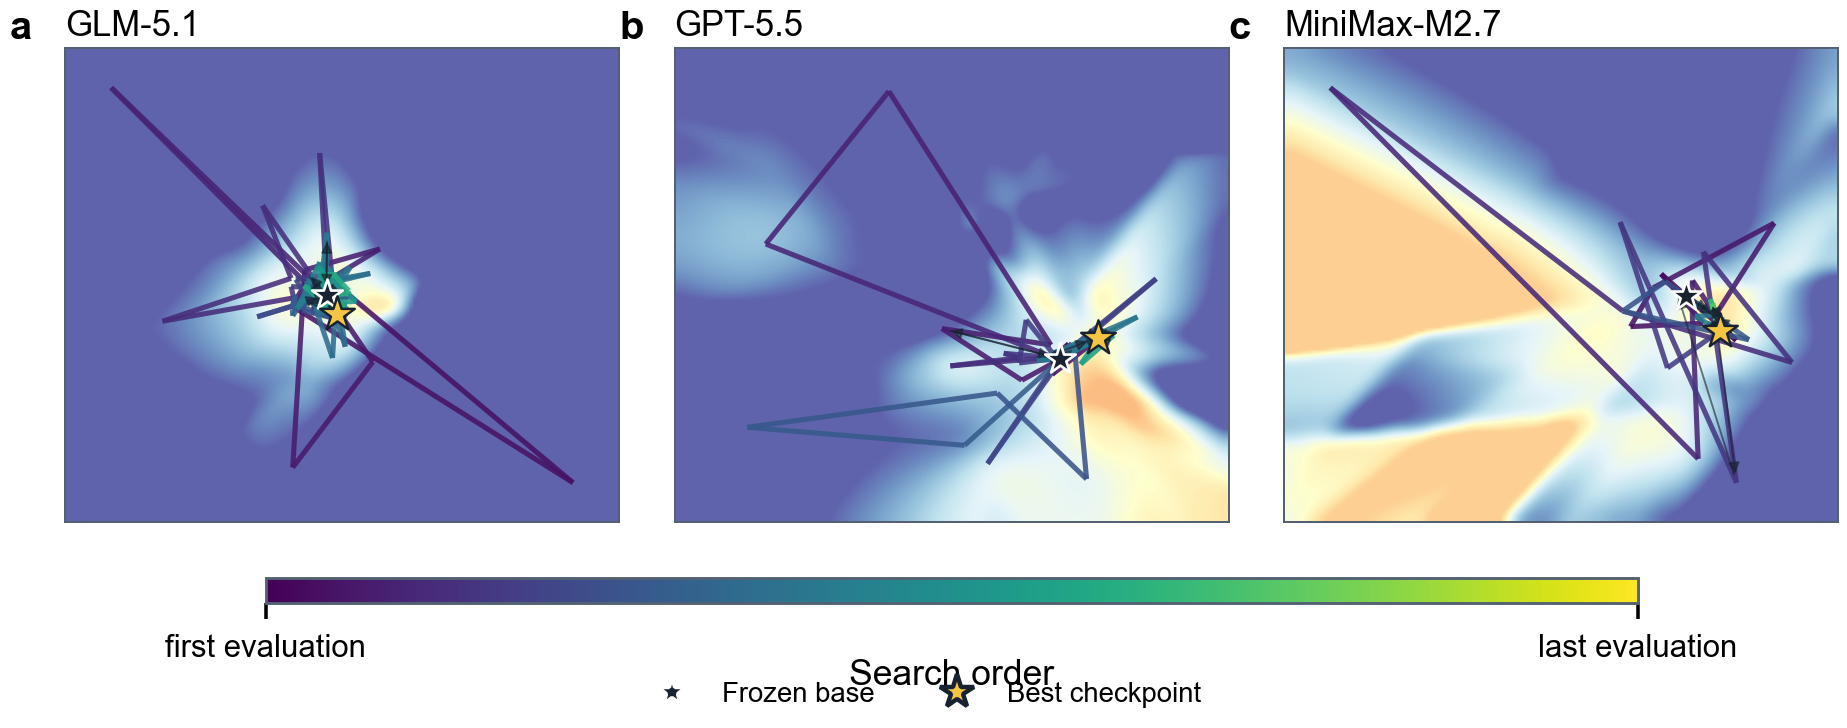
\includegraphics[width=\linewidth]{figures/fig7-weight-space-walks.pdf}
    \caption{\textbf{Complete projected weight-space walks.} Each panel is one of the three
    valid Qwen3-4B-Base episodes for which complete checkpoint programs were retained. The
    background is an interpolated visualization of
    scores actually measured in that run (blue: lower; white: near base; red: higher).
    Line color runs from the first to the last evaluation and arrows show direction. The
    black star is the frozen checkpoint, and the
    gold star is the best measured checkpoint. Panels autoscale so short walks remain
    visible; backgrounds should not be compared as calibrated global loss surfaces.}
    \label{fig:walks}
\end{figure}

The score trajectories provide a second view. Some agents evaluate independent multi-scale
batches around the base; others repeatedly perturb the incumbent or compare positive and
negative directions before moving the center. Figure~\ref{fig:trajectory} shows one
representative audit-valid run for every configuration with a detailed trace, selected as
the run closest to that configuration's median endpoint. The paths differ in candidate
coverage, the timing of improvements, and the duration of plateaus even when their
endpoints are similar.

\begin{figure}[t]
    \centering
    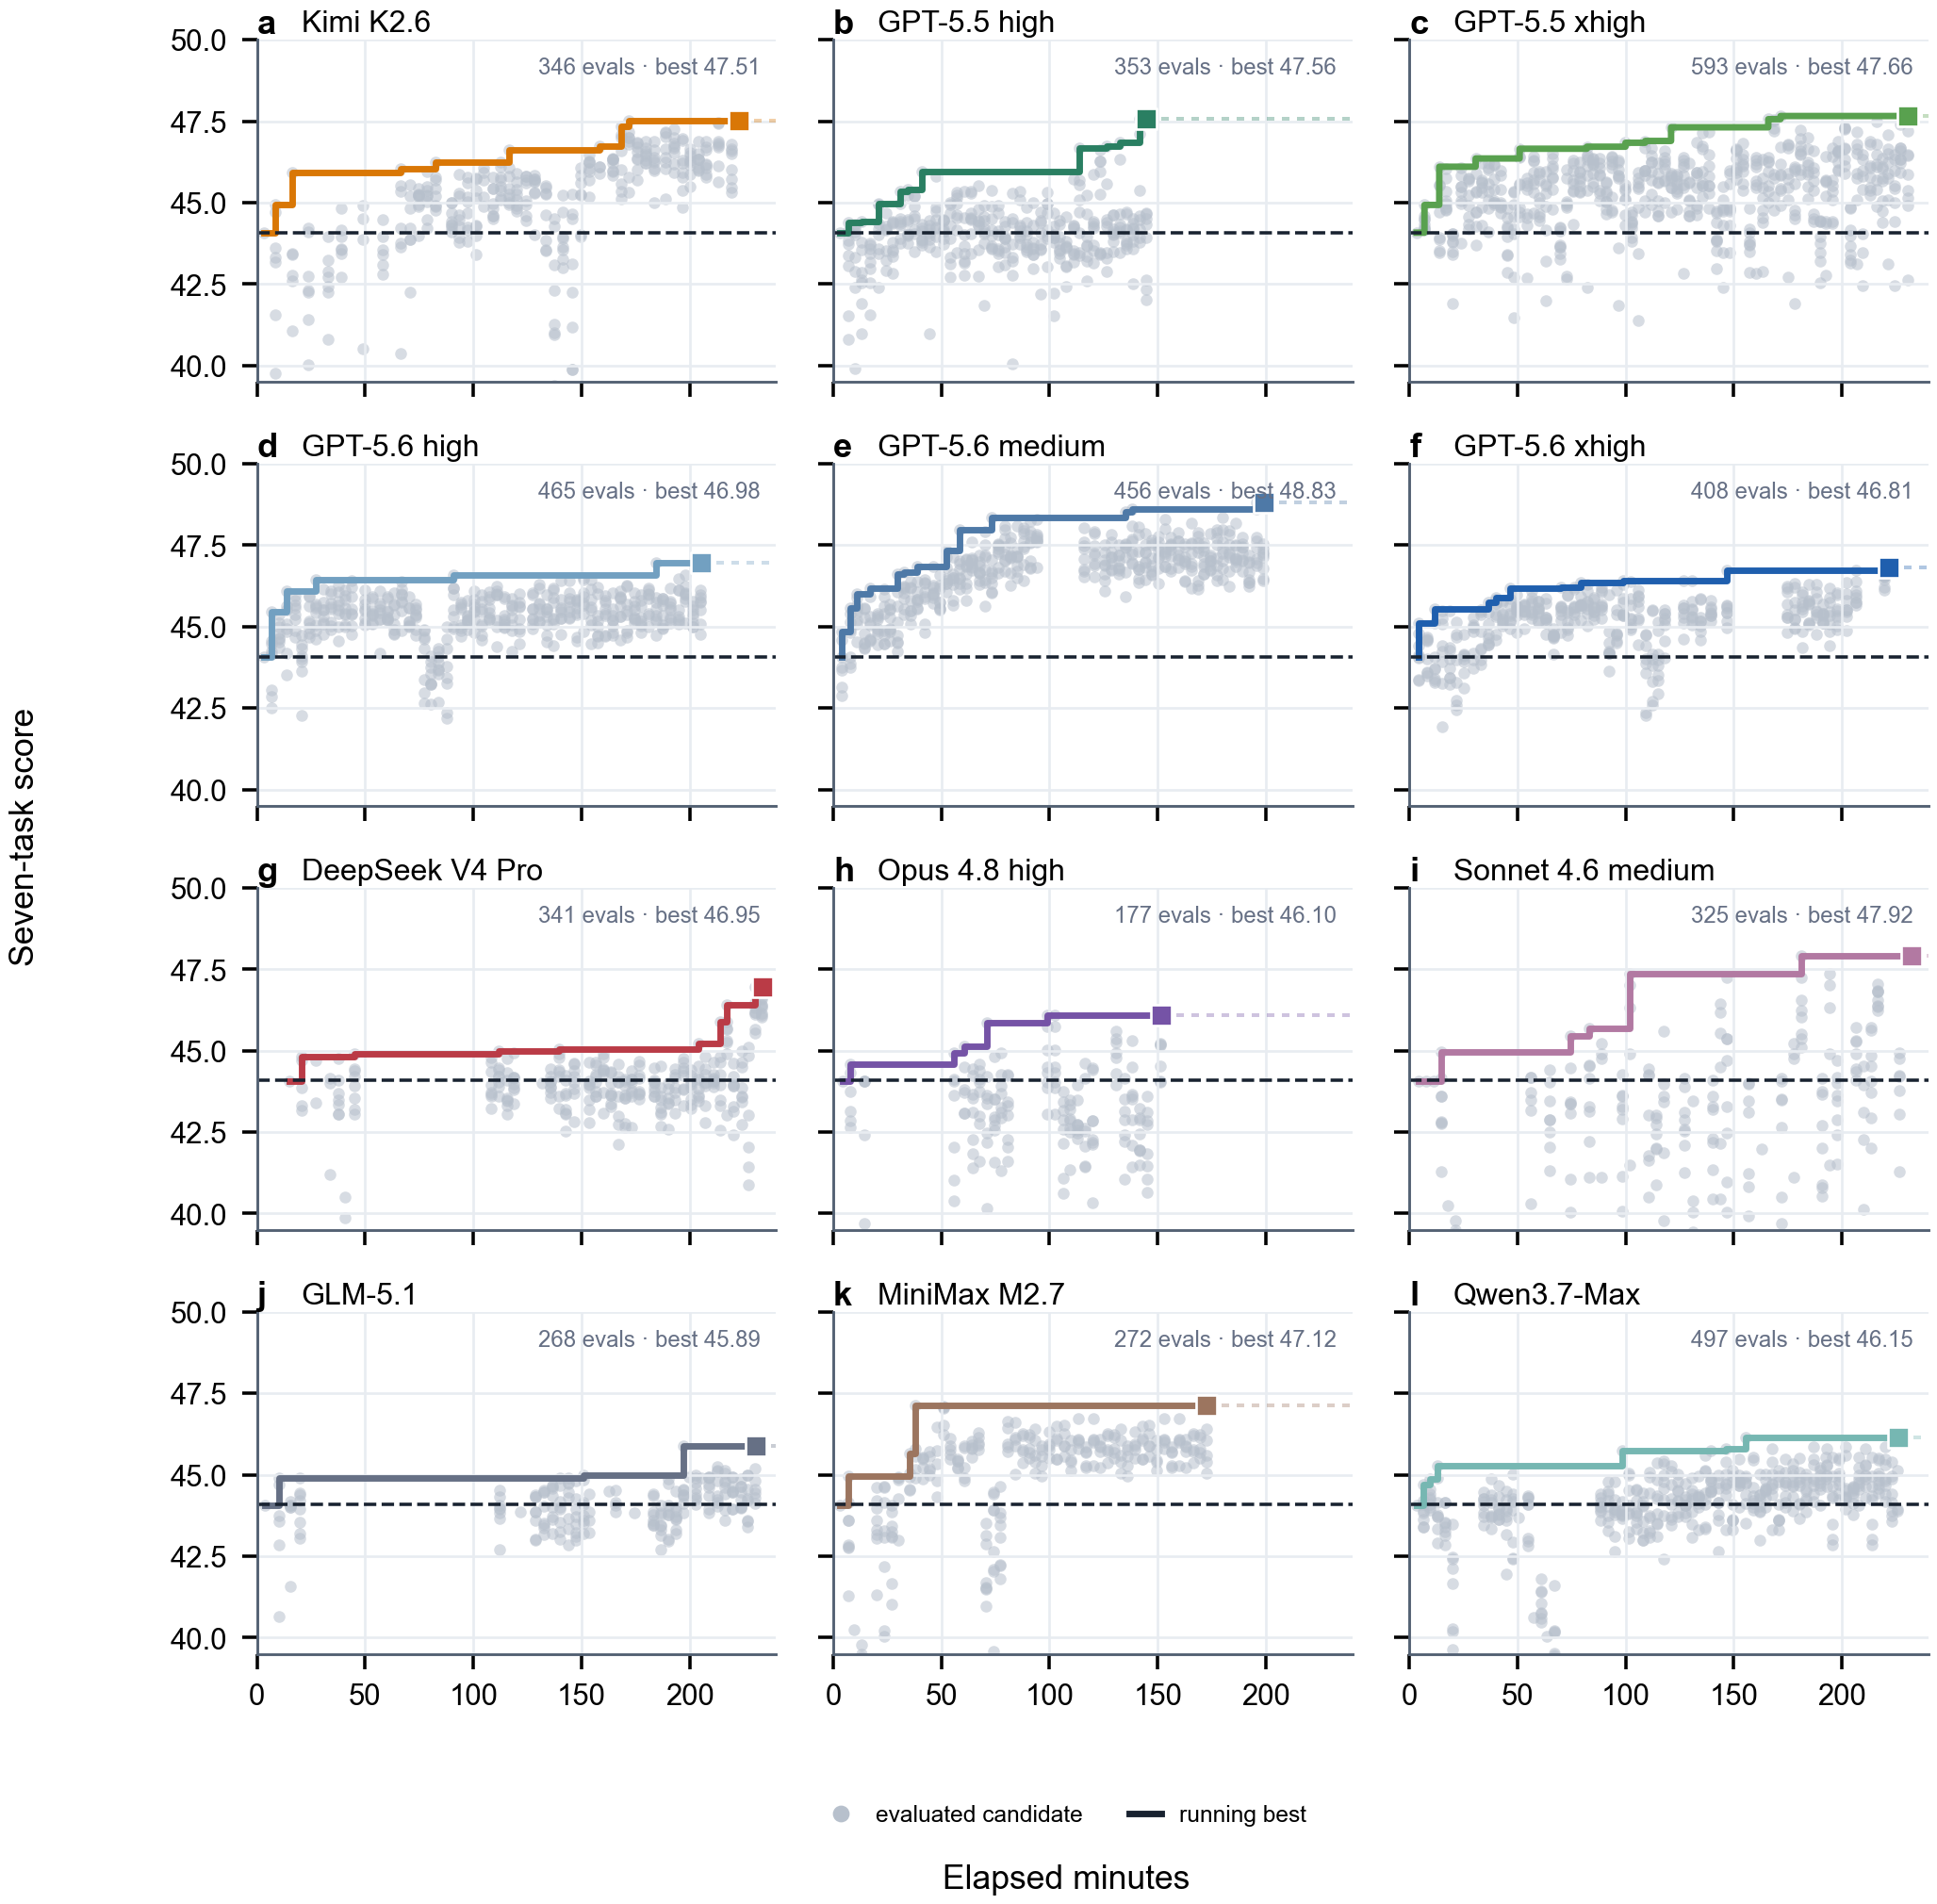
\includegraphics[width=\linewidth]{figures/fig5-trace-cases.pdf}
    \caption{\textbf{Four-hour trajectories for every configuration with complete detailed
    traces.} Gray points are retained candidate evaluations and colored steps are the
    running best. Each panel displays the audit-valid run closest to that configuration's
    median endpoint; the upper-right annotation reports the repetition count, candidate
    evaluations in the displayed run, and final best score.}
    \label{fig:trajectory}
\end{figure}

\subsection{Historical optimizer diagnostics}

Random-500 is the primary baseline in Table~\ref{tab:main}. Separately, historical
calibration runs on Qwen2.5-3B provide diagnostic evidence about optimizer sensitivity. Three
360-evaluation RandOPT runs reach 45.81--46.41. A conservative-step evolution-strategy
calibration reaches 54.68, whereas its original step setting reaches only 44.97. These
calibrations use different budgets and earlier protocol versions, so they are not baselines
in the main comparison. They nevertheless establish two facts: a fixed optimizer can exceed
the current agent endpoints, and changing only the update scale can move the same optimizer
from near-base performance to the strongest historical result. The benchmark is therefore
not a contest between ``agents'' and ``randomness.'' It asks whether an agent can discover,
implement, and manage the algorithmic choices that fixed optimizers encode by hand. A
definitive leaderboard must compare them under matched evaluation budgets and protocol
versions.

\section{Related Work}

\paragraph{Agents for machine learning and post-training research.}
MLAgentBench frames research as repeated repository modification, execution, and feedback
\citep{huang2023mlagentbench}. MLE-bench broadens the setting to end-to-end Kaggle
competitions and measures engineering outcomes against human competition baselines
\citep{chan2024mlebench}. Later work formalizes these agents as search policies over
candidate programs and shows that operator choice and search policy interact strongly
\citep{toledo2025airesearchagents}. \bench{} shares the long-horizon code-and-experiment
loop but restricts the artifact being optimized: every valid action must ultimately define
one checkpoint derived from a frozen base model. PostTrainBench evaluates autonomous
post-training on one benchmark with a ten-hour H100 budget \citep{rank2026posttrainbench}.
RSIBench-Data controls the training stack and studies
iterative data design \citep{meng2026rsibenchdata}. AI4AI-Bench freezes research
repositories and scores agent-written changes to training algorithms
\citep{chi2026ai4aibench}. These benchmarks expose complementary research variables:
PostTrainBench gives broad autonomy, RSIBench-Data isolates data strategy, and AI4AI-Bench
isolates the learning algorithm. \bench{} isolates score-driven parameter search without
backpropagation. The target model is distinct from the research agent, so the setting is
AI-for-AI experimentation rather than literal self-improvement.

\paragraph{Zeroth-order and weight-space model optimization.}
Zeroth-order methods optimize from function evaluations rather than analytic gradients
\citep{liu2020primer}. Evolution strategies estimate directions from population scores and
parallelize naturally \citep{salimans2017es}. MeZO adapts two-point gradient estimation to
fine-tune language models in place using only forward passes \citep{malladi2023mezo}, while
Agentic ESOpt applies online reward-weighted parameter updates to long-horizon agents
\citep{zheng2026agenticesopt}. These works design a particular optimizer. \bench{} instead
holds the score interface fixed and evaluates whether a general-purpose research agent can
choose, implement, and revise the optimizer during an episode. Model soups average
independently fine-tuned checkpoints that occupy a shared low-error
basin \citep{wortsman2022modelsoups}, and task arithmetic adds or subtracts directions
derived from trained task checkpoints \citep{ilharco2022taskarithmetic}. Evolutionary model
merging searches automatically over parameter-space and data-flow merging recipes
\citep{akiba2024evolutionarymerging}. Neural Thickets studies a different source of useful
directions: random perturbations around one pretrained checkpoint
\citep{gan2026neuralthickets}. \bench{} starts from this single-checkpoint setting, forbids
external expert checkpoints, and treats the agent's sequence of probes, compositions, and
code revisions as the object being evaluated.

\paragraph{Adaptive evaluation.}
Repeatedly selecting candidates using feedback from one fixed dataset creates an adaptive
data-analysis problem even when the optimizer never receives gradients. Reusing a holdout
adaptively can overfit the holdout itself \citep{dwork2015adaptive}, and leaderboard work
has studied how repeated submissions bias observed maxima \citep{blum2015ladder}. In
\bench, this issue appears at two levels: more candidate evaluations increase the expected
best-of-run score, and the agent can adapt its search policy to the same visible task views.
We therefore distinguish deterministic checkpoint replay from hidden-data generalization.

\section{Limitations and Next Protocol}

The current study is a benchmark proposal and validity experiment. First, the same 200
examples per task provide search feedback and final scores. The results measure visible
optimization, not transfer to unseen data. Second, candidate counts differ across agents,
so endpoint quality mixes search policy with system throughput. Third, most settings have
three primary runs and only two target-ablation runs; these samples are insufficient for
precise variance estimates, and selecting the top three historical primary scores is
deliberately descriptive rather than an unbiased estimator. Fourth, the Qwen3 target-model ablation changes model
family, instruction tuning, and local geometry at once; it diagnoses target sensitivity
but does not identify which factor causes it. Fifth, the candidate language restricts edits to deterministic
full-model Gaussian directions and their linear combinations; it does not yet measure
general layer-selective, sparse, low-rank, or merge-based model surgery.

A stronger protocol should add a one-shot hidden split, match completed-evaluation budgets,
run at least three successful repetitions for every agent--target pair, and compare agents
against equal-budget random search, RandOPT, evolution strategies, and a human-designed
structured method. It should report visible endpoint, hidden transfer, best-so-far area,
candidate count, accelerator time, and audit status as separate quantities. These controls
would turn the observed variation from an uncontrolled confound into a measurable property
of long-horizon agentic search.

\section{Conclusion}

\bench{} turns gradient-free weight search into a concrete agent research task. Across 39
balanced primary score-bearing runs and 16 target-model runs, every tested setting reaches
a better joint checkpoint. A stricter subset of 31 audit-valid Qwen2.5 runs provides
inspectable search trajectories and freshly replayed endpoints. The controlled search study explains the task's
structure: nearby improvements are common, task directions conflict, and finite adaptive
search creates best-of-run variation. The auxiliary Qwen3 experiment adds a separate
finding---the same agents enter a more permissive neighborhood and their ordering changes.
Together, these results provide an executable AI-for-AI environment and identify the
budget, trajectory, composition, and target controls needed for reliable comparison.

\appendix
\section{Qwen3-4B-Base Target Ablation}
\label{app:qwen3}

\begin{table}[h]
\centering
\small
\setlength{\tabcolsep}{5pt}
\caption{Auxiliary Qwen3-4B-Base results (0--100). Each exact setting contributes its two
available same-protocol score-bearing runs.}
\begin{tabular}{llrrrr}
\toprule
Agent & Harness & Mean & $\Delta$ Base & Range & $n$ \\
\midrule
MiniMax M2.7 & OpenCode & \textbf{49.00} & \textbf{+7.92} & 48.94--49.07 & 2 \\
Kimi K2.6 & OpenCode & 48.91 & +7.83 & 45.88--51.94 & 2 \\
GPT-5.4 Pro & OpenCode & 48.55 & +7.47 & 47.20--49.89 & 2 \\
DeepSeek V4 Pro & OpenCode & 48.25 & +7.17 & 46.29--50.21 & 2 \\
GPT-5.6 xhigh & Codex & 48.24 & +7.16 & 43.29--53.19 & 2 \\
GLM-5.1 & OpenCode & 45.71 & +4.63 & 44.74--46.67 & 2 \\
GPT-5.5 xhigh & Codex & 45.19 & +4.11 & 42.96--47.42 & 2 \\
Qwen3.7-Max & OpenCode & 44.50 & +3.42 & 44.38--44.62 & 2 \\
\emph{Base checkpoint} & -- & 41.08 & 0.00 & -- & -- \\
\bottomrule
\end{tabular}
\end{table}

\bibliography{references}
\bibliographystyle{iclr2026_conference}
\end{document}
